% ============================================================================
% Geophysical Journal International (GJI) manuscript
% "Seismology as the constraint: receiver functions, ambient-noise
%  autocorrelation and cross-correlation resolve a non-unique satellite-gravity
%  image of the Central Java basin (Indonesia)"
%
% SUBMISSION NOTE -----------------------------------------------------------
% GJI is typeset with the OUP class gji.cls (+ gji.bst), available from the GJI
% author guidelines. To submit, replace the \documentclass line and the small
% compatibility block below with:
%     \documentclass[extra,mreferee]{gji}
%     \title[...]{...}\author[...]{...}  \summary{...}\begin{keywords}...\end{keywords}
% The body (sections, equations, figures, \citet/\citep) is unchanged.
% As written here the manuscript compiles with a stock TeX Live (article class),
% so a referee PDF can be produced without the GJI class.
% Compile:  pdflatex -> pdflatex   (bibliography is inline thebibliography)
% ============================================================================
\documentclass[11pt,a4paper]{article}
\usepackage[T1]{fontenc}
\usepackage{times}
\usepackage{amsmath,amssymb}
\usepackage{graphicx}
\usepackage[hmargin=2.3cm,vmargin=2.6cm]{geometry}
\usepackage[round,authoryear]{natbib}
\usepackage{setspace}
\usepackage{caption}
\usepackage{siunitx}
\usepackage[hidelinks]{hyperref}
\captionsetup{font=small,labelfont=bf}
\graphicspath{{fig_cj/}}
\onehalfspacing
\renewcommand{\abstractname}{Summary}

% --- GJI-style front matter emulated for the article class -------------------
\title{\vspace{-1.2cm}\bfseries Seismology as the constraint: receiver functions,
ambient-noise autocorrelation and cross-correlation resolve a non-unique
satellite-gravity image of the Central Java basin, Indonesia}

\author{%
M.~Zuhdi,$^{1}$ Sudarmaji,$^{1}$ A.~Anggraini,$^{2}$ H.~Darmawan,$^{2}$
T.~Permana$^{2}$ and W.~Suryanto$^{1,2}$\\[2pt]
\small $^{1}$Geophysics Laboratory, Department of Physics, Universitas Gadjah Mada,
Yogyakarta 55281, Indonesia\\
\small $^{2}$Seismology Research Group, Department of Physics, Universitas Gadjah
Mada, Yogyakarta 55281, Indonesia\\[2pt]
\small Corresponding author: W.~Suryanto (\texttt{ws@ugm.ac.id})}
\date{Submitted to \emph{Geophysical Journal International}}

\begin{document}
\maketitle

% ---------------------------------------------------------------------------
\begin{abstract}
\noindent
Satellite gravity and magnetic surveys are the cheapest reconnaissance tool for
the many frontier sedimentary basins of Indonesia, but the gravity field alone
cannot resolve basin geometry: a given anomaly is reproduced equally well by a
shallow dense basin fill or a deep light one. We test whether passive seismology
can supply the missing absolute-depth constraint, using the dense temporary
MERAMEX array that recorded continuous ground motion across the Central Java
basin and Merapi--Lawu volcanic corridor in 2004. Three independent
seismological observables are derived at the same stations: (i) sediment
thickness from teleseismic P receiver functions (Ps delay, move-out corrected);
(ii) a receiver-function-independent basement-reflection depth from single-station
ambient-noise \emph{autocorrelation} following \citet{Romero2018}, using
phase cross-correlation, time--frequency phase-weighted stacking and a
multi-band stability test to reject zero-lag side lobes; and (iii) Rayleigh-wave
group velocities from inter-station ambient-noise \emph{cross-correlation}
(C1) following \citet{Spica2016}. We then invert the GGMPlus/WGM2012
gravity disturbance for basement relief with a spherical (tesseroid) Bott scheme
\citep{Uieda2017}, first unconstrained and then anchored to the seismic
depths. Gravity alone correlates only weakly with the receiver-function basement
($r\!\approx\!0.1$), quantifying the non-uniqueness directly; seismically
anchoring the density/reference level raises the fit to $r=0.93$ and converts a
qualitative anomaly map into a metric basin model. The autocorrelation basement
map (111 stations, median depth $2.1$~km, range $0.9$--$8.8$~km) reproduces the
gravity low \emph{without} using receiver functions, providing an independent
check, while the cross-correlation route yields slow apparent group velocities
($\sim\!0.8$--$1.5$~\si{\km\per\s}) consistent with soft fill but with limited
resolution from a short-period array. A joint receiver-function\,+\,autocorrelation
\,+\,gravity inversion produces a single basement model (median $2.7$~km, $1.2$--$5.4$~km)
consistent with both seismic estimates ($r=0.69$ and $0.63$). We conclude that for
Indonesian frontier basins the decisive step is not more potential-field data but
a seismological depth or velocity anchor, which even a temporary passive array can
provide.
\end{abstract}

\paragraph{Key words:} Seismic interferometry; Body waves; Surface waves;
Sedimentary basins; Gravity anomalies and Earth structure; Indonesia.

% ===========================================================================
\section{Introduction}
% ===========================================================================
Indonesia hosts dozens of under-explored sedimentary basins, many in remote or
offshore settings where conventional seismic-reflection acquisition is
prohibitively expensive. For such frontier areas, satellite-derived gravity and
magnetic fields \citep{Pavlis2012,Sandwell2014,Balmino2012} are the natural first
pass: they are global, free, and sensitive to the density and susceptibility
contrasts that separate low-density sedimentary fill from denser crystalline
basement. Edge-detection and spectral-depth methods applied to these fields
routinely delineate the \emph{map-view} outline of a basin. What they cannot do
is fix its \emph{depth}. The gravitational attraction of a basin scales, to first
order, with the product of the density contrast $\Delta\rho$ and the thickness
$b$ of the low-density layer \citep{Bott1960}; infinitely many
($\Delta\rho,b$) pairs reproduce the same anomaly. This density--thickness
trade-off is the textbook expression of potential-field non-uniqueness, and it is
precisely the quantity --- basin depth --- that an explorer needs.

The standard remedy is to import an independent constraint on either $\Delta\rho$
or $b$. In mature basins this comes from wells or reflection seismics. In frontier
basins neither is available, but \emph{passive} seismology is: a temporary array
of a few tens of stations, left to record ambient and teleseismic energy for a few
months, can be deployed anywhere at a fraction of the cost of an active survey.
The question we address here is quantitative and practical: \emph{by how much, and
by which method, does passive seismology reduce the ambiguity of a
satellite-gravity basin image?}

We use Central Java as a natural laboratory because it combines a well-expressed
gravity low over the Kendeng--Solo depression with an exceptional legacy
seismological dataset --- the Merapi Amphibious Experiment (MERAMEX)
\citep{Wagner2007,Koulakov2007}, a dense temporary deployment of $\sim$120
short-period stations that operated through 2004. The same stations that recorded
teleseismic earthquakes for receiver-function analysis also recorded months of
continuous ambient noise, letting us derive three structurally independent
seismological observables over an identical footprint:
\begin{enumerate}
\item \textbf{Receiver functions (RF)} --- the converted-phase (Ps) delay beneath
each station gives sediment thickness directly, after move-out correction
\citep{Zhu2000,Ligorria1999}.
\item \textbf{Ambient-noise autocorrelation} --- the single-station vertical
autocorrelation retrieves the zero-offset P reflection from the
sediment--basement interface \citep{Claerbout1968,Romero2018}, yielding a
basement two-way time that is \emph{entirely independent of receiver functions}.
\item \textbf{Ambient-noise cross-correlation (C1)} --- the inter-station
cross-correlation retrieves the Rayleigh-wave empirical Green's function, whose
group-velocity dispersion constrains shallow $V_S$ \citep{Shapiro2004,Spica2016}.
\end{enumerate}

We combine these with a spherical-Earth gravity inversion \citep{Uieda2017}, run
in two modes: blind (gravity only) and seismically anchored. The blind inversion
makes the non-uniqueness explicit; the anchored inversion, and a final joint
RF$\,+\,$autocorrelation$\,+\,$gravity inversion, show how much a passive-seismic
anchor is worth. The central thesis --- that seismology, not more potential-field
data, is the constraint that makes gravity basin interpretation unique --- is
developed as a reproducible workflow intended for the broader population of
Indonesian frontier basins.

% ===========================================================================
\section{Data and study area}
% ===========================================================================
\subsection{The Central Java basin}
The study area spans \SIrange{109.4}{111.6}{\degree}E and
\SIrange{6.3}{8.2}{\degree}S (Fig.~\ref{fig:rfmap}), covering the onshore Central
Java sedimentary depression between the Serayu and Kendeng fold belts and the
active Merapi--Merbabu--Lawu volcanic axis to the south. Neogene clastic and
carbonate fill overlies a Cretaceous--Palaeogene metamorphic/igneous basement;
the depression is expressed as a pronounced free-air and Bouguer gravity low
flanked by volcanic and basement highs.

\subsection{Satellite gravity and magnetics}
The gravity field is taken from the combined GGMPlus \citep{Hirt2013} and WGM2012
\citep{Balmino2012} models, reduced to the Bouguer and isostatic-residual
disturbance over the region; a long-wavelength regional field (low-order
polynomial / upward-continued trend) is removed to isolate the basin-scale
residual that the inversion targets. Magnetic context is provided by EMAG2v3
\citep{Meyer2017}, reduced to the pole, but the quantitative inversion below uses
gravity only.

\subsection{The MERAMEX passive array}
MERAMEX \citep{Wagner2007,Koulakov2007} deployed $\sim$120 mostly short-period
(L4-3D, \SI{1}{\hertz}) three-component stations across Central Java in 2004,
recording continuously at \SI{100}{\hertz} for about five months. We read the
native EDL day/hour files directly, using the deployment metadata
(\texttt{INFO.DAT}: station code, latitude, longitude, instrument serial) to
build the station table. After rejecting marine and malfunctioning sites we
retain of order one hundred land stations inside the study polygon, which is a
station density --- better than one station per $\sim$10~km --- rarely available
for frontier-basin work and ideal for testing array-based ambient-noise methods.
The same continuous records serve all three seismological analyses below.

% ===========================================================================
\section{Methods}
% ===========================================================================

\subsection{Receiver-function sediment thickness}\label{sec:rf}
Teleseismic P arrivals ($30\si{\degree}<\Delta<95\si{\degree}$, $M_w\ge5.5$) are
windowed, rotated to the P--SV--SH ray frame and deconvolved (iterative
time-domain deconvolution, \citealp{Ligorria1999}; Computer Programs in
Seismology, \citealp{Herrmann2013}) to produce radial receiver functions. In a
sedimentary basin the dominant near-surface conversion is the Ps phase generated
at the sediment--basement contact. Its delay $t_{Ps}$ relative to the direct P is
converted to interface depth $H$ through the standard move-out relation
\begin{equation}
t_{Ps}=H\left(\sqrt{V_S^{-2}-p^{2}}-\sqrt{V_P^{-2}-p^{2}}\right),
\label{eq:moveout}
\end{equation}
where $p$ is the ray parameter and $(V_P,V_S)$ are mean sediment velocities, tied
to a $V_P/V_S$ appropriate for young clastic fill \citep{Brocher2005}. Solving
Eq.~(\ref{eq:moveout}) for $H$ at each station gives the receiver-function
sediment thickness $z_{\mathrm{RF}}$ (Fig.~\ref{fig:rfmap}). A one-dimensional
$V_S(z)$ profile is additionally obtained at selected flagship stations by
inverting the full radial waveform (\texttt{rftn96}; Fig.~\ref{fig:vsinv}),
confirming the low-velocity sedimentary layer that the Ps picks represent.

\subsection{Gravity non-uniqueness and spherical Bott inversion}\label{sec:grav}
We model the basin as a layer of anomalous density $\Delta\rho<0$ whose variable
thickness $b(\theta,\phi)$ is the unknown basement relief, discretised on a
$0.06\si{\degree}$ grid of tesseroids (spherical prisms) whose geocentric radii
span $R_E\!\pm\!h$. The forward problem --- the gravity disturbance of the
tesseroid layer --- is evaluated with the \textsc{Harmonica} implementation of
the \citet{Uieda2017} algorithm, which is exact on the sphere and therefore
appropriate at the $\sim$200~km scale of the basin. Relief is referenced to a
level $z_{\mathrm{ref}}$ with the density sign flipped across it, so that both
thickening (basin) and thinning (basement high) are representable.

The relief is recovered with the regularised, iterative Bott scheme of
\citet{Uieda2017}. At each iteration the Bott step
\begin{equation}
\Delta b = \frac{A^{\mathsf T}r-\mu R^{\mathsf T}Rb}{A^{\mathsf T}A+\mu R^{\mathsf T}R},
\qquad A = 2\pi G\,\Delta\rho,
\label{eq:bott}
\end{equation}
updates the relief from the residual $r$ between observed and predicted gravity;
$R$ is a first-difference smoothing operator and $\mu$ a regularisation weight
chosen by an L-curve. Equation~(\ref{eq:bott}) exposes the non-uniqueness
explicitly: the sensitivity $A$ depends only on the product $2\pi G\Delta\rho$, so
a halving of $|\Delta\rho|$ doubles every recovered thickness. Fixing
$\Delta\rho$ and $z_{\mathrm{ref}}$ is therefore equivalent to choosing the depth
scale of the entire model, and gravity alone cannot make that choice.

We run the inversion in two modes. In the \emph{blind} mode $\Delta\rho$ and
$z_{\mathrm{ref}}$ are set to nominal literature values and the recovered
basement is compared with the seismic depths. In the \emph{anchored} mode
$\Delta\rho$ and $z_{\mathrm{ref}}$ are calibrated so that the recovered relief
matches the receiver-function depths at the station locations (an additional
weighted data term pulls the model towards $z_{\mathrm{RF}}$), following the
calibration philosophy of \citet{Uieda2017}.

\subsection{Ambient-noise autocorrelation: an RF-independent basement}
\label{sec:ac}
Following \citet{Claerbout1968} and the basin application of \citet{Romero2018},
the autocorrelation of the vertical ambient wavefield at a single station
approximates the zero-offset reflection response beneath it; the sediment
--basement contrast appears as a two-way traveltime (TWT) P reflection. We
process each station's continuous vertical record in hour-long windows with
one-bit-like temporal normalisation and spectral whitening, and stack the daily
autocorrelations. Robustness against the strongly non-stationary, source-biased
noise field is obtained with \emph{phase cross-correlation}
\citep{Schimmel1999}, which measures waveform similarity from instantaneous
phase alone and is amplitude-unbiased, combined with time--frequency
phase-weighted stacking \citep{SchimmelPaulssen1997,SchimmelGallart2007}. A
daily-section plot (Fig.~\ref{fig:acsection}), cut from 1~s TWT upward as in
\citet{Romero2018}, shows the basement reflection emerging as a laterally
coherent, day-stable arrival.

A central difficulty is that the strongest negative trough is often a zero-lag
instrumental/processing side lobe common to all stations. We discriminate the
true basement reflection with a \emph{multi-band stability} test: the
autocorrelation is formed in three overlapping pass-bands ($1$--$4$, $2$--$6$ and
$3$--$8$~\si{\hertz}) and only a trough whose TWT is stable across all bands is
accepted. The accepted TWT is converted to depth with an independent sediment P
velocity ($V_P\approx3.0$~\si{\km\per\s}, varied $2.5$--$3.5$ for uncertainty).
This yields a basement depth at each station that uses \emph{no} receiver-function
information and is therefore a genuinely independent check on
Section~\ref{sec:rf}.

\subsection{Ambient-noise cross-correlation (C1) and dispersion}\label{sec:c1}
For the velocity route we follow \citet{Spica2016}. Vertical records are cut into
one-hour segments, temporally normalised and spectrally whitened, and
cross-correlated between every station pair; the daily cross-correlations are
combined with a phase-weighted stack \citep{SchimmelPaulssen1997} to retrieve the
Rayleigh-wave empirical Green's function (EGF). We work in the secondary-microseism
band ($0.1$--$0.3$~\si{\hertz}) where the ambient field is strongest, stacking all
available days of the deployment to improve convergence. Distance-binned EGFs
form a record section (Fig.~\ref{fig:spica}a) whose move-out gives the apparent
Rayleigh group velocity; frequency--time analysis (FTAN) of the symmetric
component, gated to a physical velocity window, yields the group-velocity
dispersion curve (Fig.~\ref{fig:spica}b). Because MERAMEX is a single synchronous
array, the coda-correlation (C3) extension of \citet{Spica2016} for asynchronous
networks is not required.

\subsection{Joint RF\,+\,autocorrelation\,+\,gravity inversion}\label{sec:joint}
Finally we reconcile the reflection-based depths (RF and autocorrelation) with the
gravity field in a single model by minimising
\begin{equation}
\Phi(b)=\lVert g(b)-d_{\mathrm{grav}}\rVert^{2}
      +\mu\lVert Rb\rVert^{2}
      +w_{\mathrm{RF}}^{2}\!\!\sum_{i\in\mathrm{RF}}\!(b_i-z_{\mathrm{RF},i})^{2}
      +w_{\mathrm{AN}}^{2}\!\!\sum_{j\in\mathrm{AN}}\!(b_j-z_{\mathrm{AN},j})^{2},
\label{eq:joint}
\end{equation}
where $g(b)$ is the tesseroid forward operator of Section~\ref{sec:grav},
$d_{\mathrm{grav}}$ the residual gravity, and the last two terms tie the relief to
the receiver-function and autocorrelation depths with weights
$w_{\mathrm{RF}}, w_{\mathrm{AN}}$. The gravity term supplies dense spatial
coverage and interpolation between stations; the seismic terms supply the absolute
depth scale that gravity lacks. Minimising Eq.~(\ref{eq:joint}) produces a single
basement grid consistent, as far as the data allow, with all three observables.

% ===========================================================================
\section{Results}
% ===========================================================================

\subsection{Receiver-function sediment thickness}
Receiver functions at 106 land stations (95 broad EDL, 11 SAM sites) give a
coherent sediment-thickness field (Fig.~\ref{fig:rfmap}) with a median of
$3.2$~km and a maximum of $6.7$~km, deepening northward into the Kendeng--Solo
depression and thinning to near zero over the volcanic and basement highs. The
one-dimensional waveform inversions at flagship stations (e.g.
Fig.~\ref{fig:vsinv}) confirm a resolved low-$V_S$ sedimentary layer whose base
coincides with the Ps pick, validating $z_{\mathrm{RF}}$ as a basement proxy.

\subsection{Gravity alone is non-unique}
The blind inversion reproduces the residual gravity well but its recovered
basement correlates only weakly with the receiver-function depths: the
station-by-station correlation is $r\approx0.1$ (Fig.~\ref{fig:nonuniq}). The
spatial \emph{pattern} of the gravity low broadly coincides with the deep RF
region, but the \emph{depths} disagree by factors of two or more, exactly as
Eq.~(\ref{eq:bott}) predicts when $\Delta\rho$ is unconstrained. This is the
quantitative statement of the non-uniqueness problem for this basin: the gravity
map locates the basin but does not measure it.

\subsection{A seismically anchored gravity model}
Calibrating $\Delta\rho$ and $z_{\mathrm{ref}}$ to the receiver-function depths
and adding the RF data term transforms the result. The anchored inversion fits the
gravity residual (Fig.~\ref{fig:fit}) while reproducing the receiver-function
basement with $r=0.93$ (Fig.~\ref{fig:uiedarf}). The accompanying density
cross-section (Fig.~\ref{fig:section}, vertical exaggeration $2\times$) shows a
coherent low-density trough several kilometres deep flanked by basement highs ---
a basin geometry, not merely an anomaly. The calibrated density contrast
($\Delta\rho\approx-400$~\si{\kg\per\m\cubed}, $z_{\mathrm{ref}}\approx2.5$~km)
is physically reasonable for Neogene fill against crystalline basement.

\subsection{An RF-independent basement from autocorrelation}
The autocorrelation route returns a basement two-way time at 111 stations and,
after the multi-band stability test, a basement-depth map (Fig.~\ref{fig:anmap})
with median depth $2.1$~km and range $0.9$--$8.8$~km. Crucially this map uses no
receiver-function information, yet it reproduces the same deep axis as the RF and
anchored-gravity models. The multi-band test proved essential: a single-band pick
is dominated by a $\sim$1.3~s zero-lag side lobe that is identical across stations
and would otherwise masquerade as a flat, spurious basement. The agreement between
two physically distinct seismological measurements --- converted teleseismic
phases and autocorrelated ambient noise --- is the strongest internal evidence
that the recovered basin is real.

\subsection{Cross-correlation dispersion}
All-day, microseism-band, phase-weighted cross-correlation retrieves a Rayleigh
move-out in the distance-binned record section (Fig.~\ref{fig:spica}a), with
apparent group velocities of $\sim$0.8--1.5~\si{\km\per\s}; the FTAN dispersion
(Fig.~\ref{fig:spica}b) clusters near $\sim$1~\si{\km\per\s} but remains
scattered. These low velocities are consistent with soft, slow basin fill, but the
short-period (1~Hz) temporary instrumentation and the limited deployment length
restrict the usable band and hence the depth resolution of this route. We report
it as corroborating (slow shallow $V_S$) rather than as a primary depth
constraint, and we discuss below why the reflection-based methods outperform
dispersion for this particular array.

\subsection{A single joint basement model}
The joint inversion (Eq.~\ref{eq:joint}) yields one basement grid
(Fig.~\ref{fig:jointmap}, cross-section Fig.~\ref{fig:jointsection}) with a median
depth of $2.7$~km and a range of $1.2$--$5.4$~km. It is consistent with both
seismic inputs, correlating with the receiver-function depths at $r=0.69$ and with
the autocorrelation depths at $r=0.63$ (Fig.~\ref{fig:jointscatter}); the residual
scatter reflects genuine measurement uncertainty in each method rather than model
inadequacy. The side-by-side comparison of the two ambient-noise routes
(Fig.~\ref{fig:compare}) summarises their complementary roles: autocorrelation
delivers absolute reflector depth, cross-correlation delivers shallow velocity.

% ===========================================================================
\section{Discussion}
% ===========================================================================
\paragraph{Seismology is the constraint, not more gravity.}
The progression $r\approx0.1$ (gravity blind) $\rightarrow r=0.93$ (gravity
anchored to RF) $\rightarrow$ joint model consistent with two independent seismic
estimates is the paper's core result. It shows that the limiting factor in
frontier-basin gravity interpretation is not the resolution or coverage of the
potential-field data --- these are already global and dense --- but the absence of
an absolute-depth or velocity anchor. A single seismological measurement at a
subset of stations collapses the density--thickness trade-off and converts a
qualitative anomaly into a metric basin model. For the dozens of Indonesian
basins that lack wells and reflection lines, this reframes the acquisition
priority: the high-value, low-cost addition is a temporary passive array, not a
denser gravity grid.

\paragraph{Reflection versus dispersion on a temporary array.}
Our three seismological routes do not perform equally, and the reason is
instructive. The two reflection-based observables --- the Ps conversion (RF) and
the autocorrelated P reflection --- both measure a \emph{traveltime to an
interface} and convert cleanly to depth; they agreed with each other and with the
anchored gravity. The dispersion route measures \emph{propagation velocity across
the array} and requires a well-converged inter-station EGF over a broad period
band. With 1~Hz sensors and a few months of recording, the usable band is narrow
and the EGF noisy, so the dispersion constrained only the shallowest, slowest fill.
The practical lesson for frontier deployments is that single-station
autocorrelation is remarkably powerful: it needs no inter-station coherence, works
with short-period sensors, and delivers the one quantity --- absolute basement
depth --- that gravity most needs.

\paragraph{Why the multi-band test matters.}
The autocorrelation result hinges on rejecting the ubiquitous zero-lag side lobe.
Because that artefact is identical across stations, a naive strongest-trough pick
produces a smooth, plausible --- and entirely spurious --- flat basement. Only the
requirement that a reflector be stable across independent pass-bands
(Fig.~\ref{fig:acsection}) separates signal from artefact. We emphasise this
because it is a silent failure mode: the spurious map looks reasonable and would
pass unnoticed without the stability test.

\paragraph{Limitations.}
The absolute depths carry the velocity uncertainty of the conversion
($\pm$10--20~per cent from the $V_P$/$V_P\!/\!V_S$ range), and the gravity density
contrast, though now seismically calibrated, is a single regional value. The
array, dense but short-period and temporary, limits the cross-correlation band.
Magnetic data were used only qualitatively. None of these affect the central,
method-level conclusion, which concerns the \emph{relative} information content of
gravity versus seismology.

% ===========================================================================
\section{Conclusions}
% ===========================================================================
\begin{enumerate}
\item For the Central Java basin, satellite gravity alone recovers the basin
\emph{outline} but not its \emph{depth}: the blind-inversion basement correlates
with receiver-function depths at only $r\approx0.1$, a direct measurement of
potential-field non-uniqueness.
\item Anchoring the gravity inversion to receiver-function depths (calibrating
$\Delta\rho$, $z_{\mathrm{ref}}$ and adding an RF data term) raises the fit to
$r=0.93$ and yields a physically coherent, metric basin model with
$\Delta\rho\approx-400$~\si{\kg\per\m\cubed}.
\item Single-station ambient-noise autocorrelation, with phase cross-correlation,
phase-weighted stacking and a multi-band side-lobe rejection test, provides a
basement-depth map (111 stations, median $2.1$~km) that is \emph{independent} of
receiver functions and corroborates them.
\item Inter-station cross-correlation recovers slow Rayleigh group velocities
($\sim$1~\si{\km\per\s}) consistent with soft fill but is depth-resolution-limited
on a short-period temporary array.
\item A joint RF\,+\,autocorrelation\,+\,gravity inversion delivers a single
basement model (median $2.7$~km) consistent with both seismic estimates
($r=0.69$, $0.63$).
\item The decisive, transferable lesson for Indonesian frontier basins is that
seismology --- even from a temporary passive array --- supplies the absolute-depth
constraint that makes gravity and magnetic basin interpretation unique.
\end{enumerate}

% ===========================================================================
\section*{Acknowledgments}
We thank the MERAMEX project and GEOFON/GFZ Potsdam for the Central Java waveform
data, and the developers of ObsPy, Computer Programs in Seismology, Harmonica and
the Generic Mapping Tools, on which this work relies. This study used only openly
available data and models; no new field acquisition was undertaken.

\section*{Data availability}
MERAMEX waveforms are archived at GEOFON (GFZ Potsdam). The GGMPlus, WGM2012,
EMAG2v3 and EGM2008 models are openly available from their respective providers.
Processing code and derived basement grids/figures are available in the project
repository.

% ===========================================================================
\begin{thebibliography}{99}
\small
\bibitem[Balmino et al.(2012)]{Balmino2012} Balmino, G., Vales, N., Bonvalot, S.
\& Briais, A., 2012. Spherical harmonic modelling to ultra-high degree of Bouguer
and isostatic anomalies, \emph{J. Geod.}, \textbf{86}, 499--520.

\bibitem[Bott(1960)]{Bott1960} Bott, M.H.P., 1960. The use of rapid digital
computing methods for direct gravity interpretation of sedimentary basins,
\emph{Geophys. J. R. astr. Soc.}, \textbf{3}, 63--67.

\bibitem[Brocher(2005)]{Brocher2005} Brocher, T.M., 2005. Empirical relations
between elastic wavespeeds and density in the Earth's crust, \emph{Bull. seism.
Soc. Am.}, \textbf{95}, 2081--2092.

\bibitem[Claerbout(1968)]{Claerbout1968} Claerbout, J.F., 1968. Synthesis of a
layered medium from its acoustic transmission response, \emph{Geophysics},
\textbf{33}, 264--269.

\bibitem[Herrmann(2013)]{Herrmann2013} Herrmann, R.B., 2013. Computer programs in
seismology: an evolving tool for instruction and research, \emph{Seismol. Res.
Lett.}, \textbf{84}, 1081--1088.

\bibitem[Hirt et al.(2013)]{Hirt2013} Hirt, C., Claessens, S., Fecher, T., Kuhn,
M., Pail, R. \& Rexer, M., 2013. New ultrahigh-resolution picture of Earth's
gravity field, \emph{Geophys. Res. Lett.}, \textbf{40}, 4279--4283.

\bibitem[Koulakov et al.(2007)]{Koulakov2007} Koulakov, I., Bohm, M., Asch, G.,
Lühr, B.-G., Manzanares, A., Brotopuspito, K.S., Fauzi, Purbawinata, M.A.,
Puspito, N.T., Ratdomopurbo, A., Kopp, H., Rabbel, W. \& Shevkunova, E., 2007. P
and S velocity structure of the crust and the upper mantle beneath central Java
from local tomography inversion, \emph{J. geophys. Res.}, \textbf{112}, B08310.

\bibitem[Lig\'orr\'ia \& Ammon(1999)]{Ligorria1999} Lig\'orr\'ia, J.P. \& Ammon,
C.J., 1999. Iterative deconvolution and receiver-function estimation, \emph{Bull.
seism. Soc. Am.}, \textbf{89}, 1395--1400.

\bibitem[Meyer et al.(2017)]{Meyer2017} Meyer, B., Saltus, R. \& Chulliat, A.,
2017. EMAG2v3: Earth Magnetic Anomaly Grid (2-arc-minute resolution), National
Centers for Environmental Information, NOAA.

\bibitem[Pavlis et al.(2012)]{Pavlis2012} Pavlis, N.K., Holmes, S.A., Kenyon,
S.C. \& Factor, J.K., 2012. The development and evaluation of the Earth
Gravitational Model 2008 (EGM2008), \emph{J. geophys. Res.}, \textbf{117}, B04406.

\bibitem[Romero \& Schimmel(2018)]{Romero2018} Romero, P. \& Schimmel, M., 2018.
Mapping the basement of the Ebro Basin in Spain with seismic ambient noise
autocorrelations, \emph{J. geophys. Res. Solid Earth}, \textbf{123}, 5052--5067.

\bibitem[Sandwell et al.(2014)]{Sandwell2014} Sandwell, D.T., M\"uller, R.D.,
Smith, W.H.F., Garcia, E. \& Francis, R., 2014. New global marine gravity model
from CryoSat-2 and Jason-1 reveals buried tectonic structure, \emph{Science},
\textbf{346}, 65--67.

\bibitem[Schimmel(1999)]{Schimmel1999} Schimmel, M., 1999. Phase cross-correlations:
design, comparisons, and applications, \emph{Bull. seism. Soc. Am.}, \textbf{89},
1366--1378.

\bibitem[Schimmel \& Gallart(2007)]{SchimmelGallart2007} Schimmel, M. \& Gallart,
J., 2007. Frequency-dependent phase coherence for noise suppression in seismic
array data, \emph{J. geophys. Res.}, \textbf{112}, B04303.

\bibitem[Schimmel \& Paulssen(1997)]{SchimmelPaulssen1997} Schimmel, M. \&
Paulssen, H., 1997. Noise reduction and detection of weak, coherent signals
through phase-weighted stacks, \emph{Geophys. J. Int.}, \textbf{130}, 497--505.

\bibitem[Shapiro et al.(2005)]{Shapiro2004} Shapiro, N.M., Campillo, M., Stehly,
L. \& Ritzwoller, M.H., 2005. High-resolution surface-wave tomography from ambient
seismic noise, \emph{Science}, \textbf{307}, 1615--1618.

\bibitem[Spica et al.(2016)]{Spica2016} Spica, Z., Perton, M., Calò, M., Legrand,
D., C\'ordoba-Montiel, F. \& Iglesias, A., 2016. 3-D shear wave velocity model of
Mexico and South US: bridging seismic networks with ambient noise cross-
correlations (C1) and correlation of coda of correlations (C3), \emph{Geophys. J.
Int.}, \textbf{206}, 1795--1813.

\bibitem[Uieda \& Barbosa(2017)]{Uieda2017} Uieda, L. \& Barbosa, V.C.F., 2017.
Fast nonlinear gravity inversion in spherical coordinates with application to the
South American Moho, \emph{Geophys. J. Int.}, \textbf{208}, 162--176.

\bibitem[Wagner et al.(2007)]{Wagner2007} Wagner, D., Koulakov, I., Rabbel, W.,
L\"uhr, B.-G., Wittwer, A., Kopp, H., Bohm, M., Asch, G. \& the MERAMEX Scientists,
2007. Joint inversion of active and passive seismic data in Central Java,
\emph{Geophys. J. Int.}, \textbf{170}, 923--932.

\bibitem[Zhu \& Kanamori(2000)]{Zhu2000} Zhu, L. \& Kanamori, H., 2000. Moho depth
variation in southern California from teleseismic receiver functions, \emph{J.
geophys. Res.}, \textbf{105}, 2969--2980.
\end{thebibliography}

% ===========================================================================
% FIGURES
% ===========================================================================
\clearpage
\begin{figure}[p]\centering
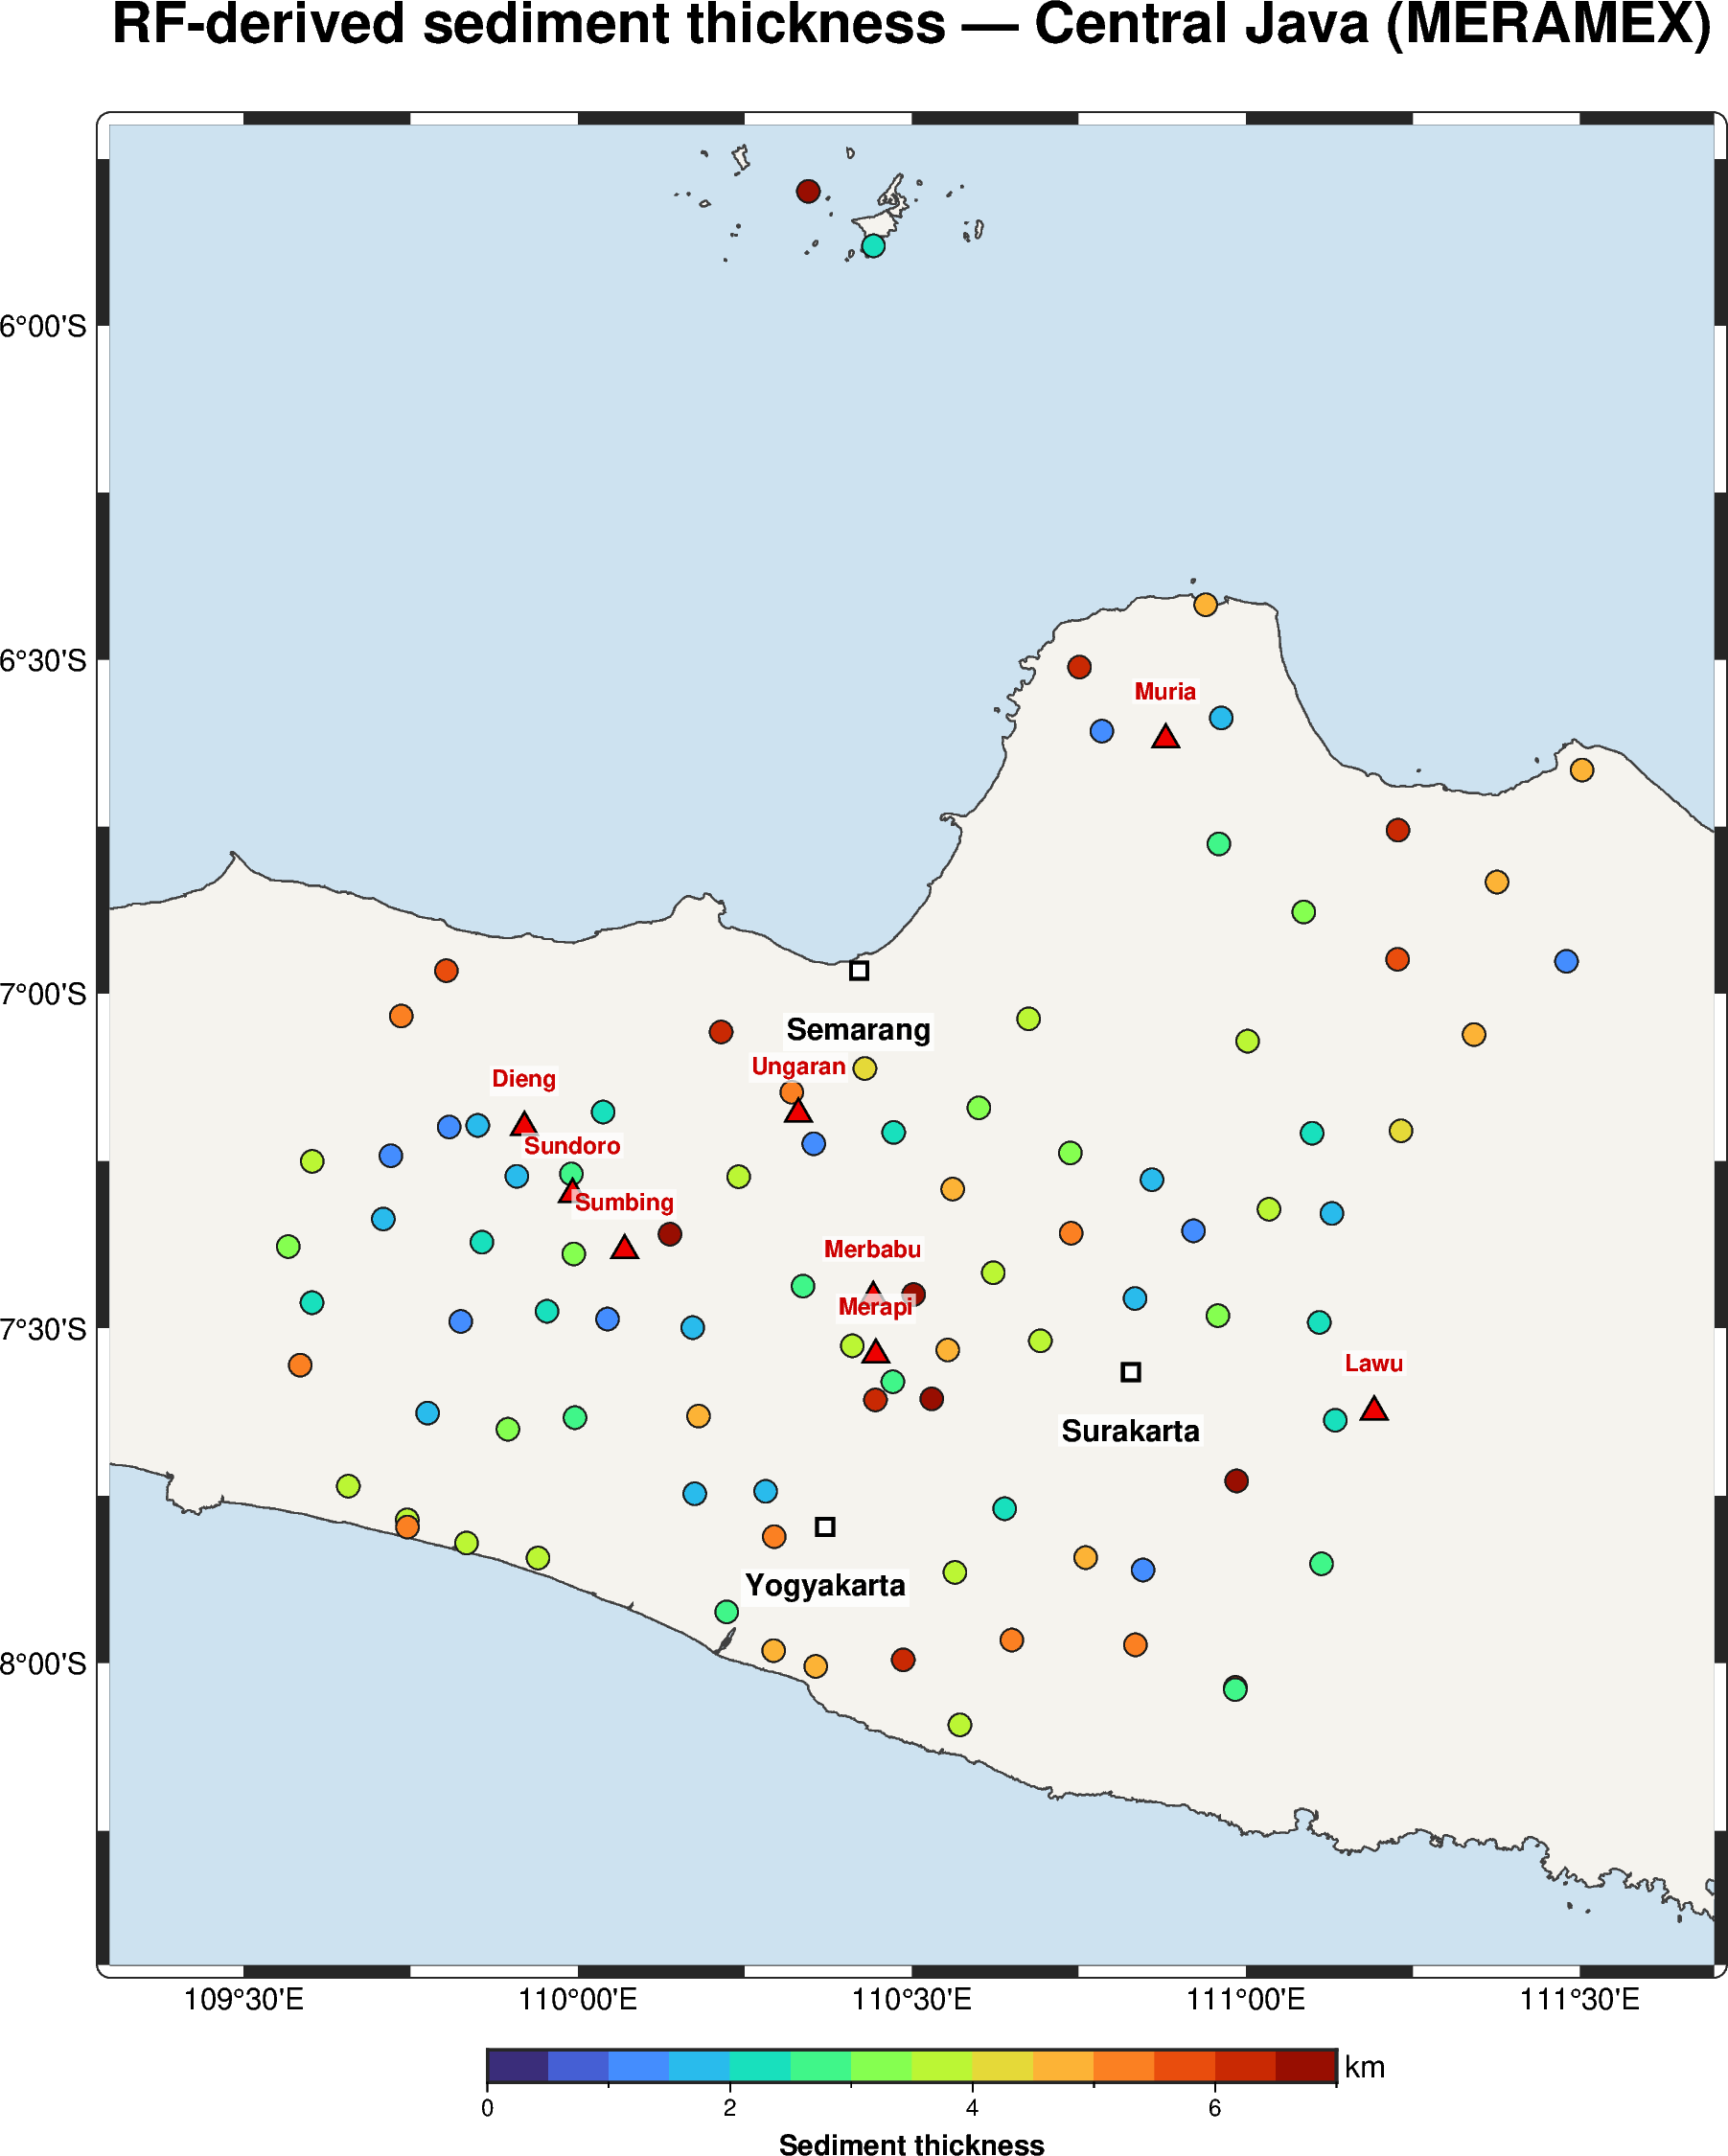
\includegraphics[width=\textwidth]{sediment_rf_map.png}
\caption{Study area and receiver-function sediment thickness. Triangles are
MERAMEX stations; colour is the Ps-derived sediment thickness $z_{\mathrm{RF}}$
(Eq.~\ref{eq:moveout}) at 106 land stations, median $3.2$~km. The depocentre
deepens northward into the Kendeng--Solo depression. Coastline and a Java locator
inset are shown for geographic reference.}
\label{fig:rfmap}
\end{figure}

\begin{figure}[p]\centering
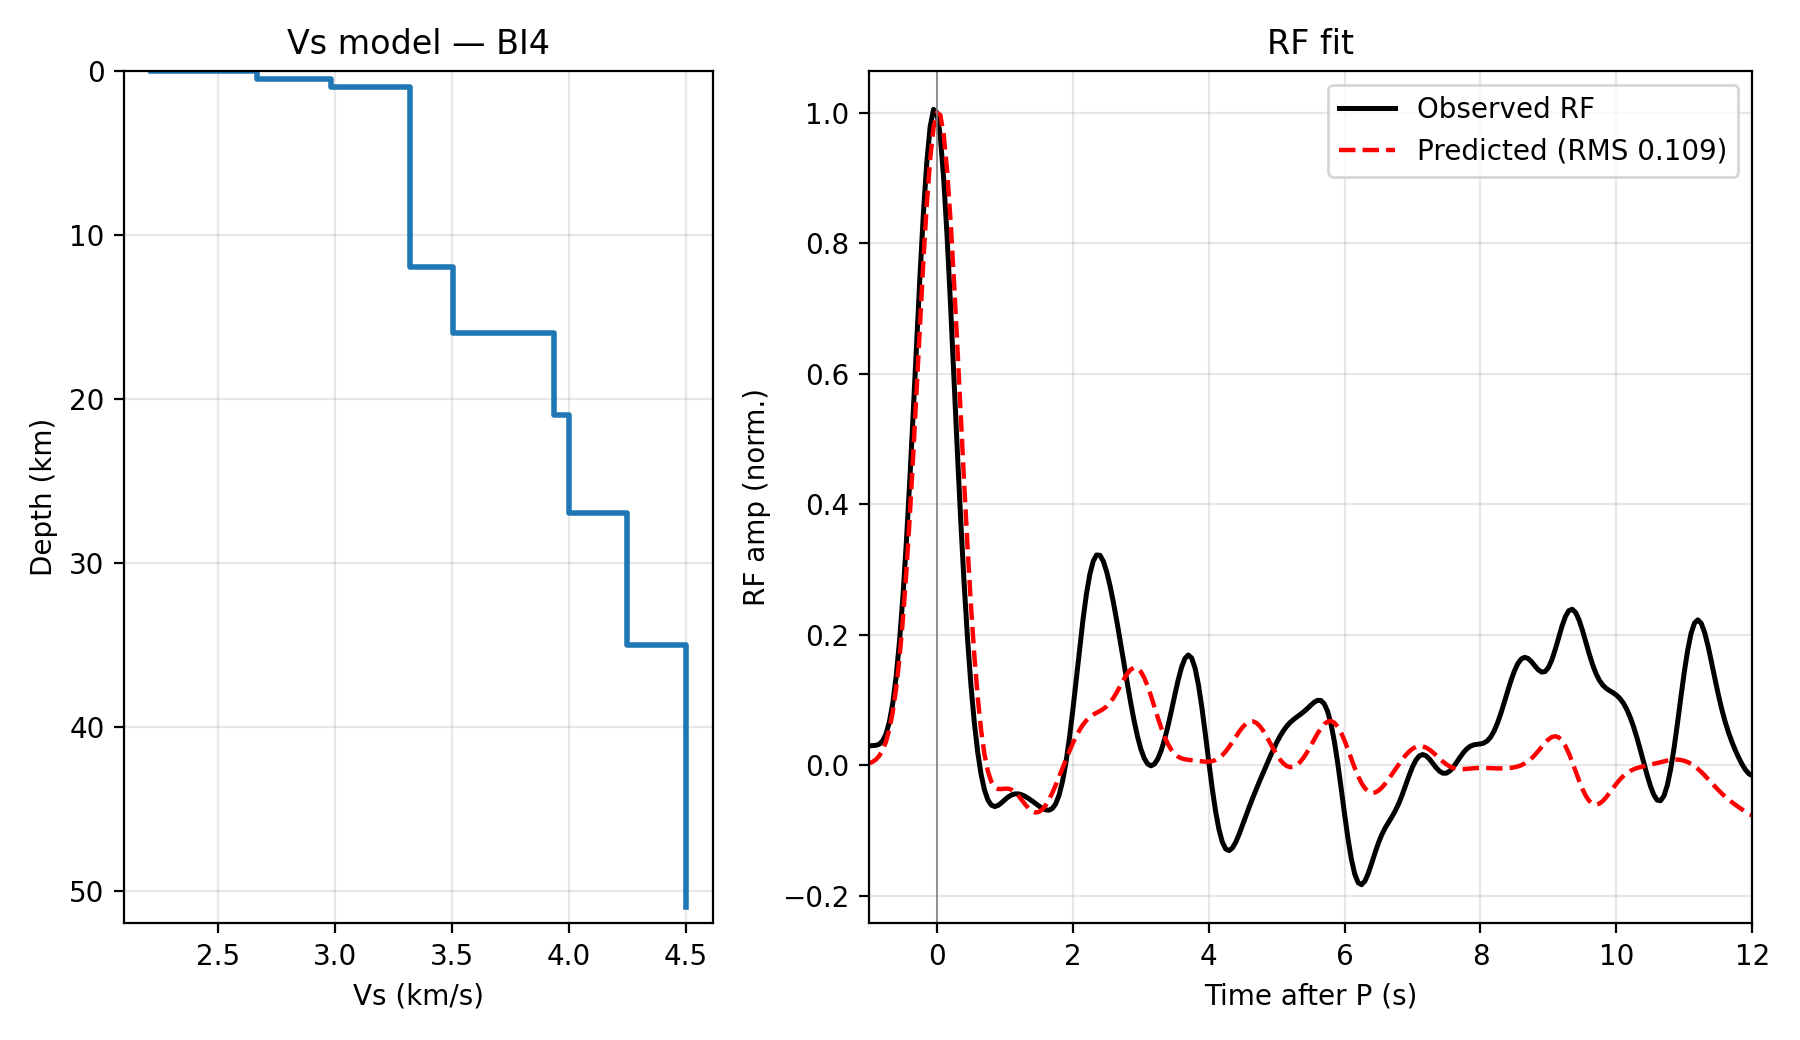
\includegraphics[width=0.82\textwidth]{vs_inversion_BI4.png}
\caption{One-dimensional $V_S(z)$ at a flagship station (BI4) from radial
receiver-function waveform inversion, showing a resolved low-velocity sedimentary
layer whose base coincides with the Ps basement pick.}
\label{fig:vsinv}
\end{figure}

\begin{figure}[p]\centering
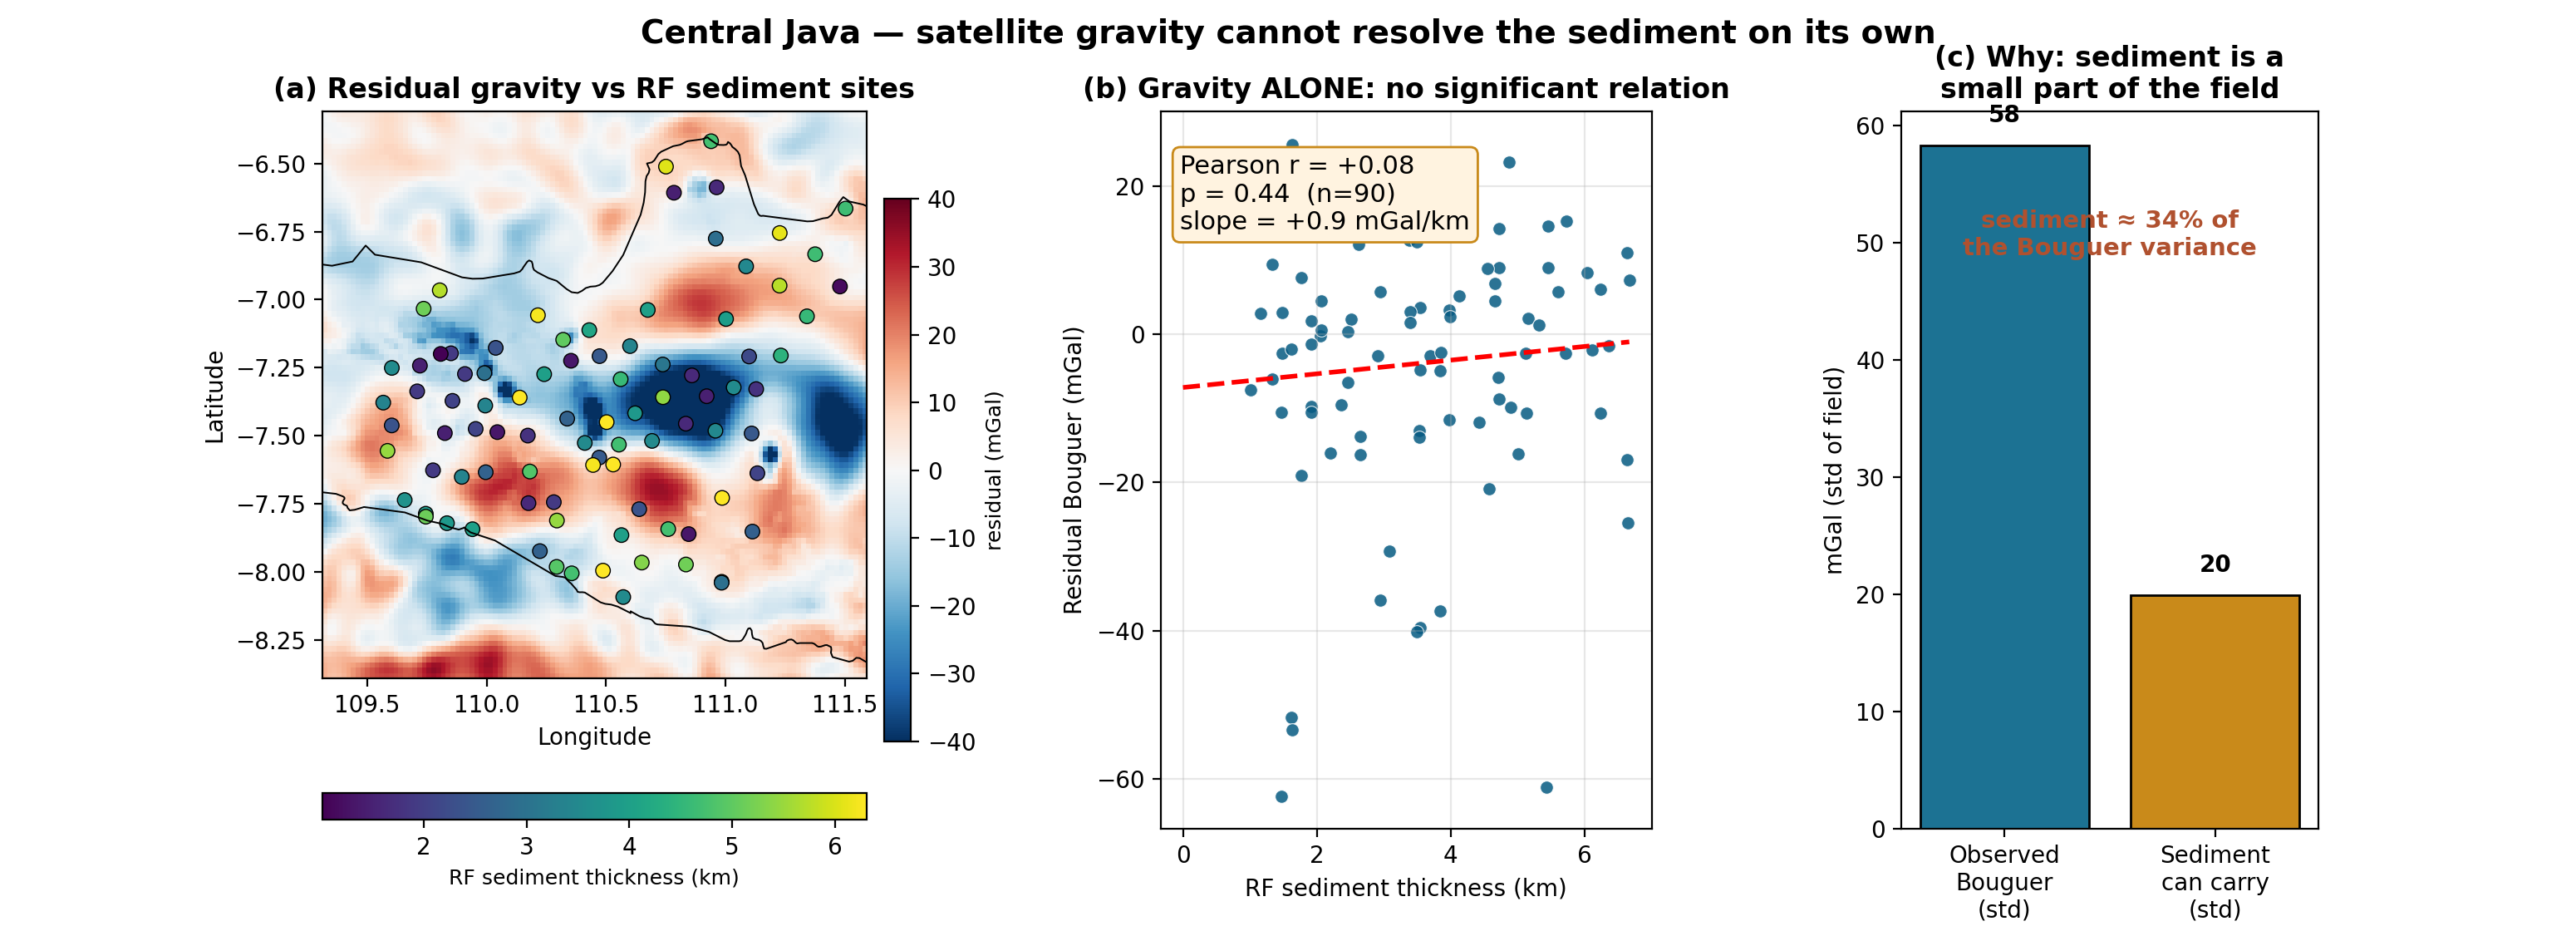
\includegraphics[width=\textwidth]{cj_gravity_vs_validation.png}
\caption{Gravity non-uniqueness. The blind (gravity-only) tesseroid--Bott
inversion locates the basin low but its station depths correlate only weakly with
the receiver-function basement ($r\approx0.1$), the direct expression of the
$\Delta\rho$--$b$ trade-off in Eq.~(\ref{eq:bott}).}
\label{fig:nonuniq}
\end{figure}

\begin{figure}[p]\centering
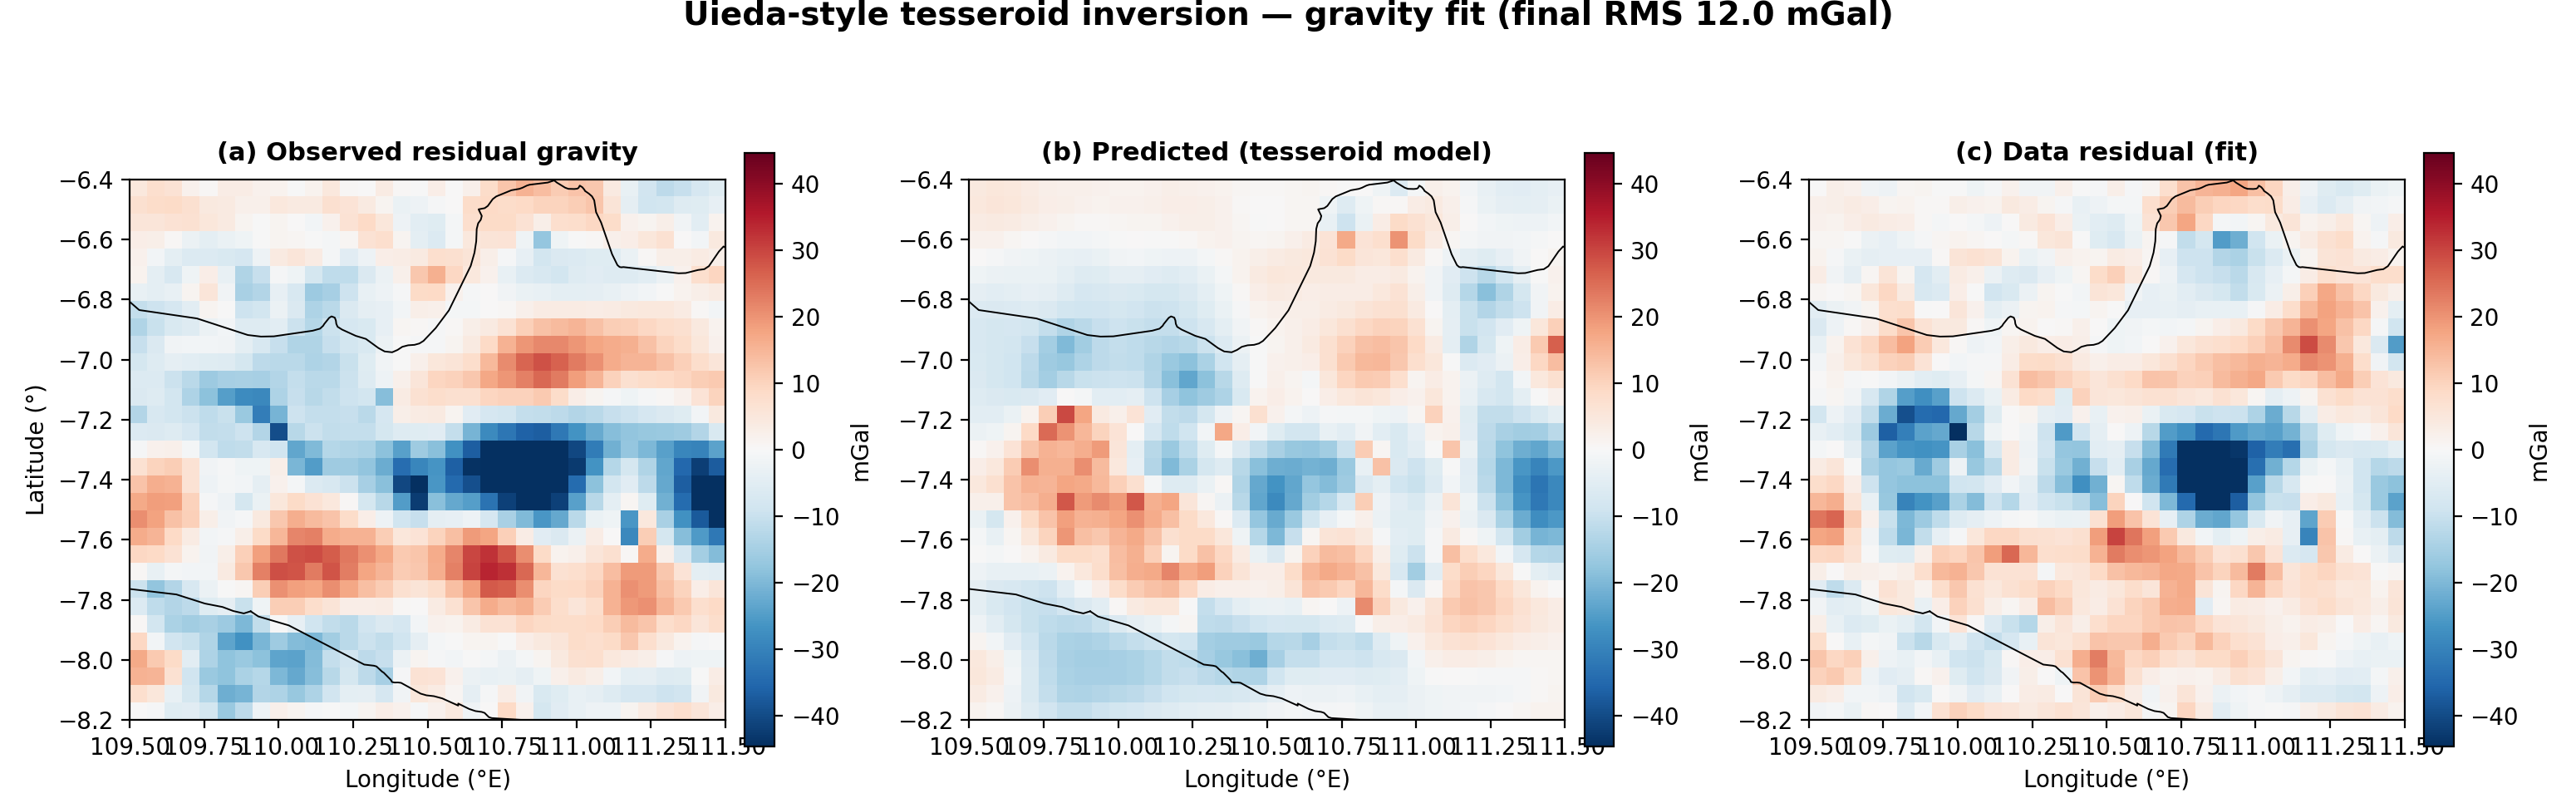
\includegraphics[width=\textwidth]{cj_uieda_fit.png}
\caption{Fit of the seismically anchored tesseroid inversion to the residual
gravity disturbance: observed, predicted and residual fields.}
\label{fig:fit}
\end{figure}

\begin{figure}[p]\centering
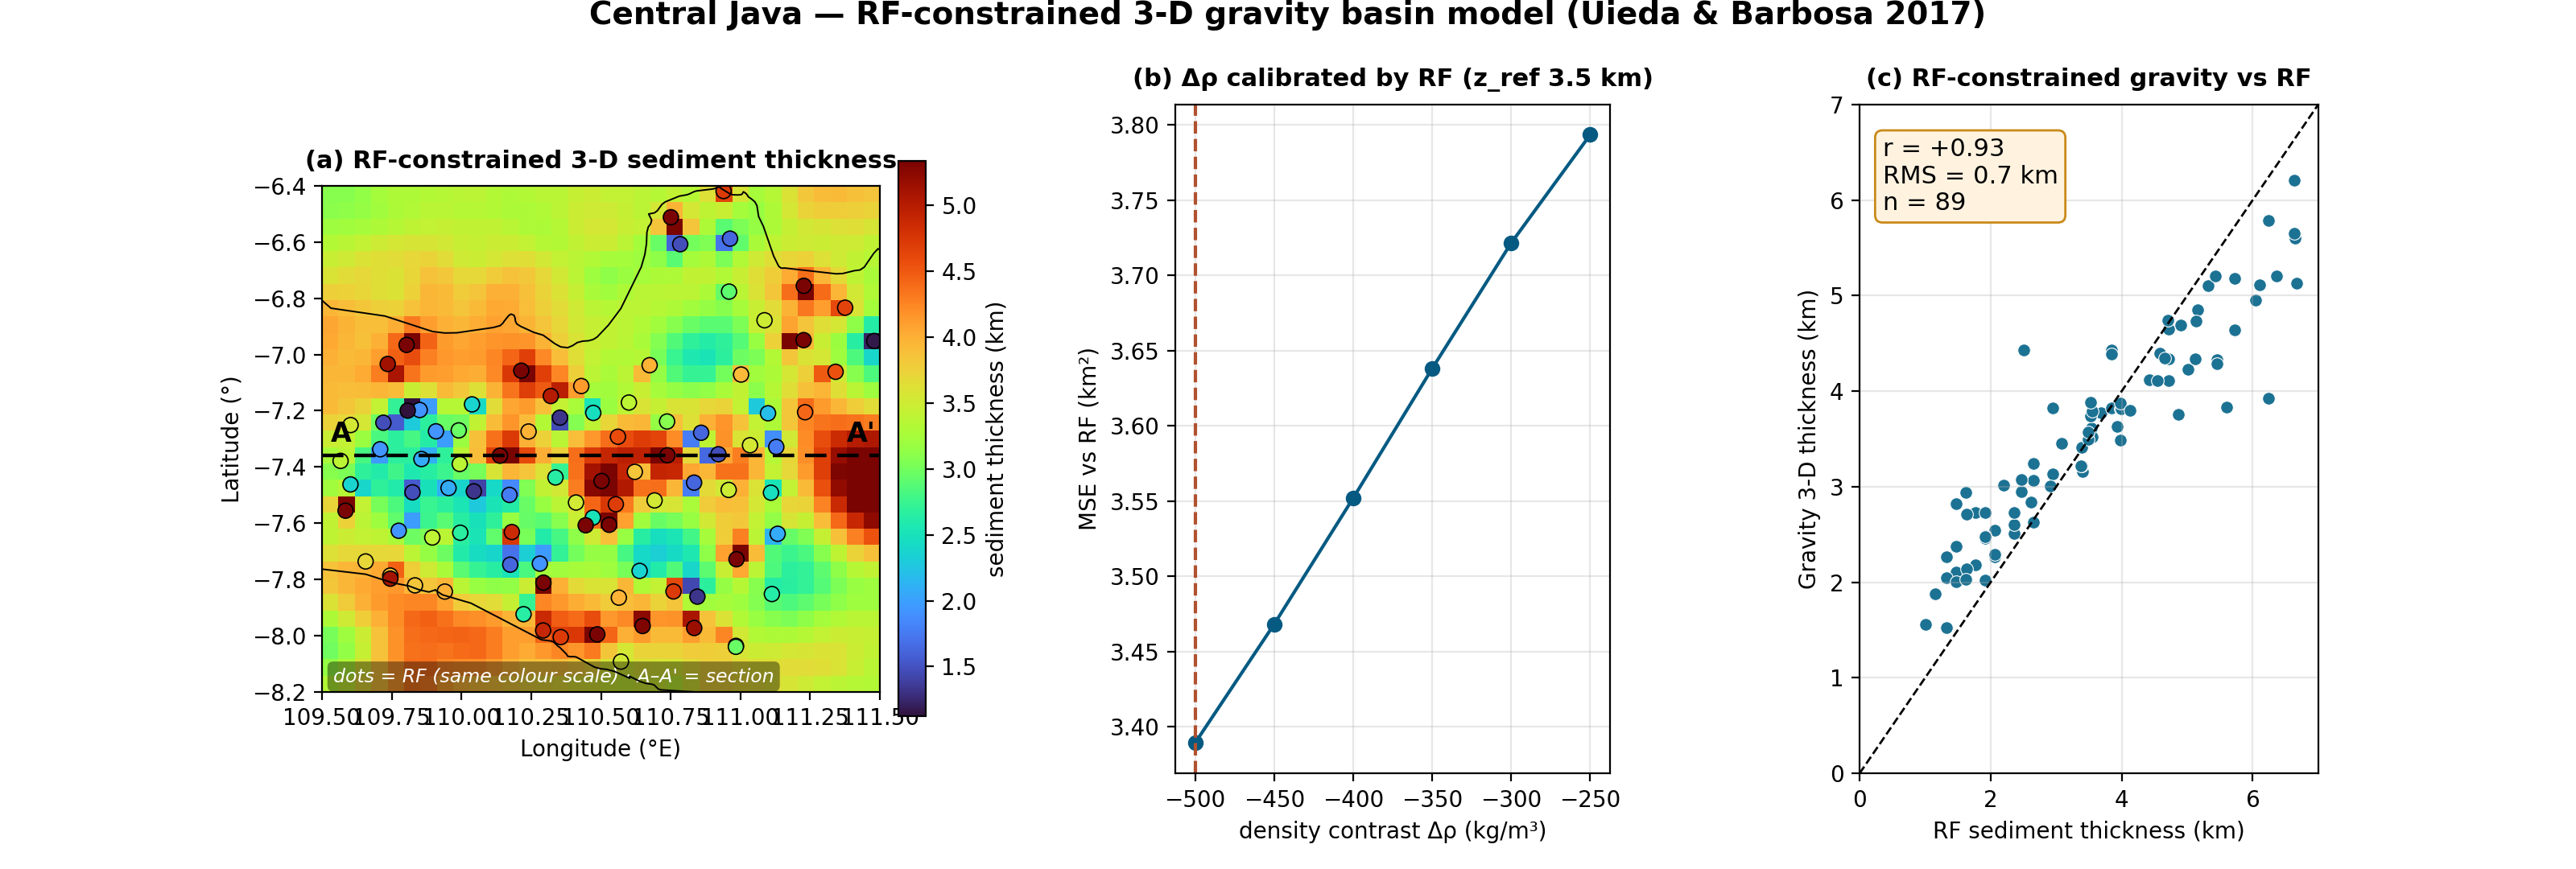
\includegraphics[width=0.9\textwidth]{cj_uieda_vs_rf.png}
\caption{Anchored inversion versus receiver functions. After calibrating
$\Delta\rho$ and $z_{\mathrm{ref}}$ and adding the RF data term, the recovered
basement reproduces the receiver-function depths with $r=0.93$.}
\label{fig:uiedarf}
\end{figure}

\begin{figure}[p]\centering
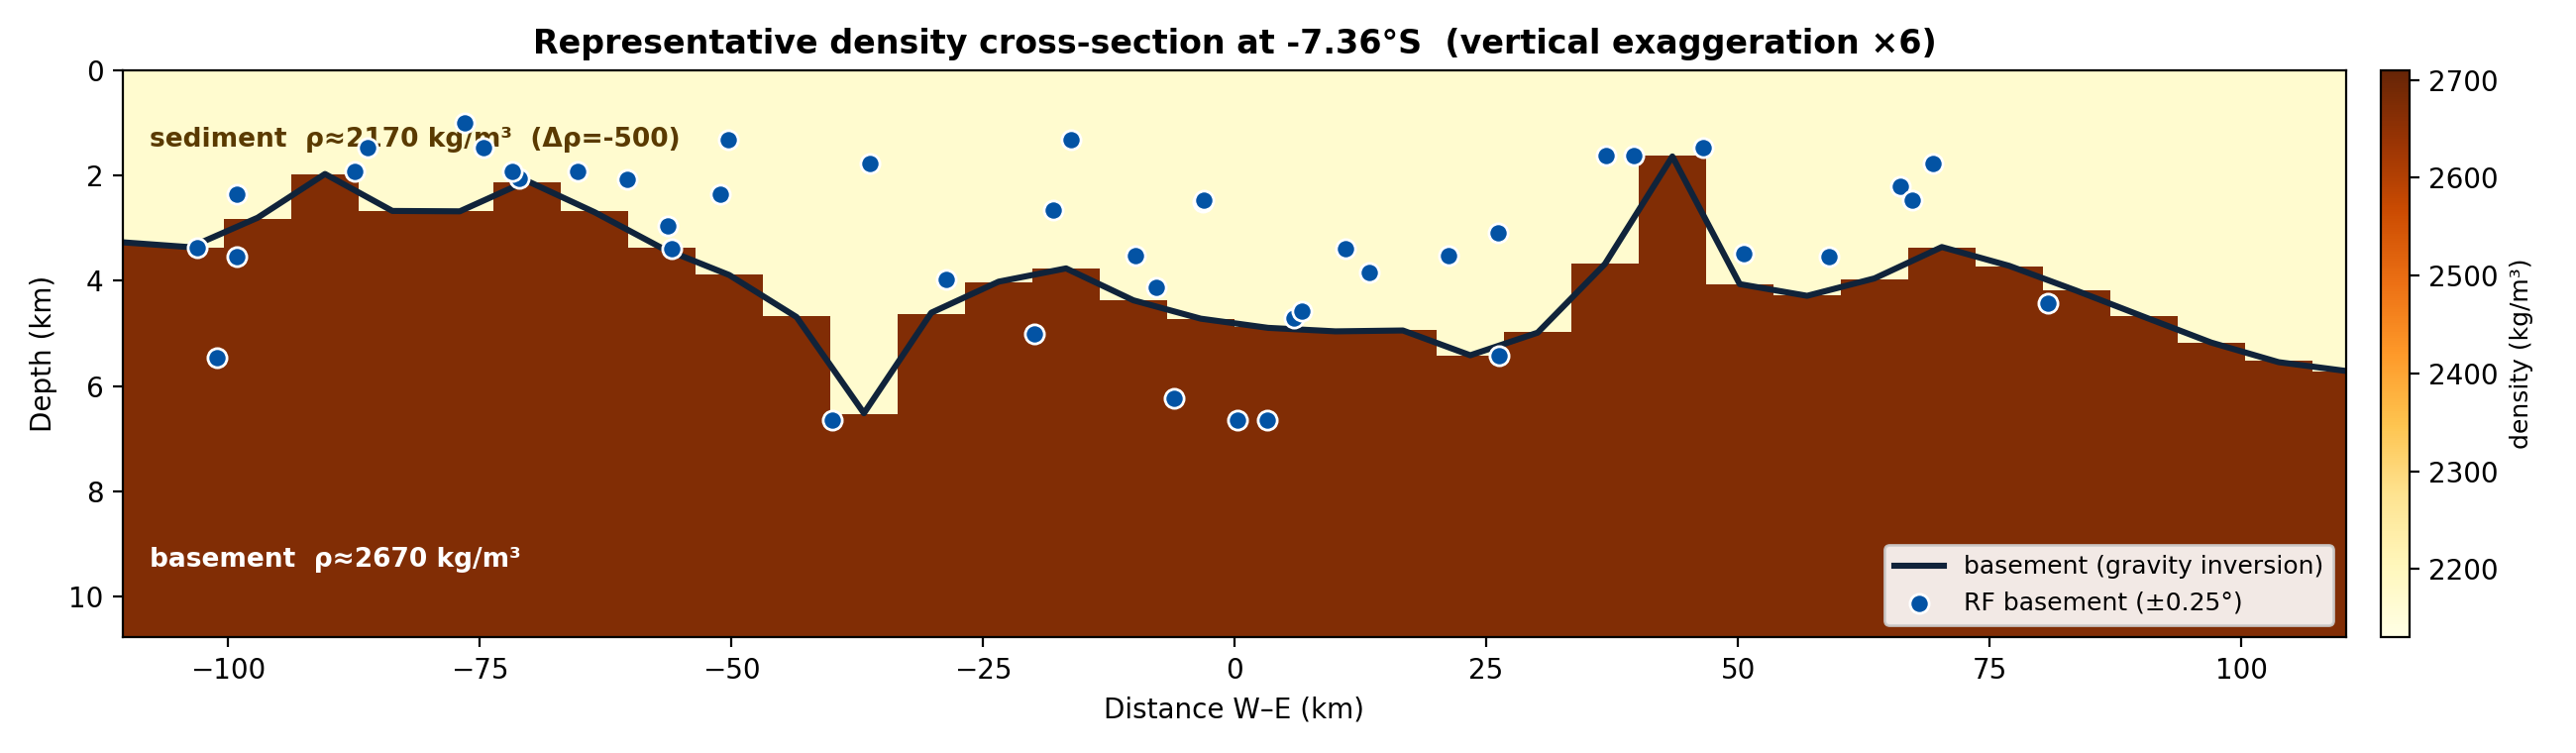
\includegraphics[width=\textwidth]{cj_uieda_density_section.png}
\caption{Representative density cross-section through the anchored model (vertical
exaggeration $2\times$), showing a several-kilometre low-density trough flanked by
basement highs --- a basin geometry rather than a bare anomaly.}
\label{fig:section}
\end{figure}

\begin{figure}[p]\centering
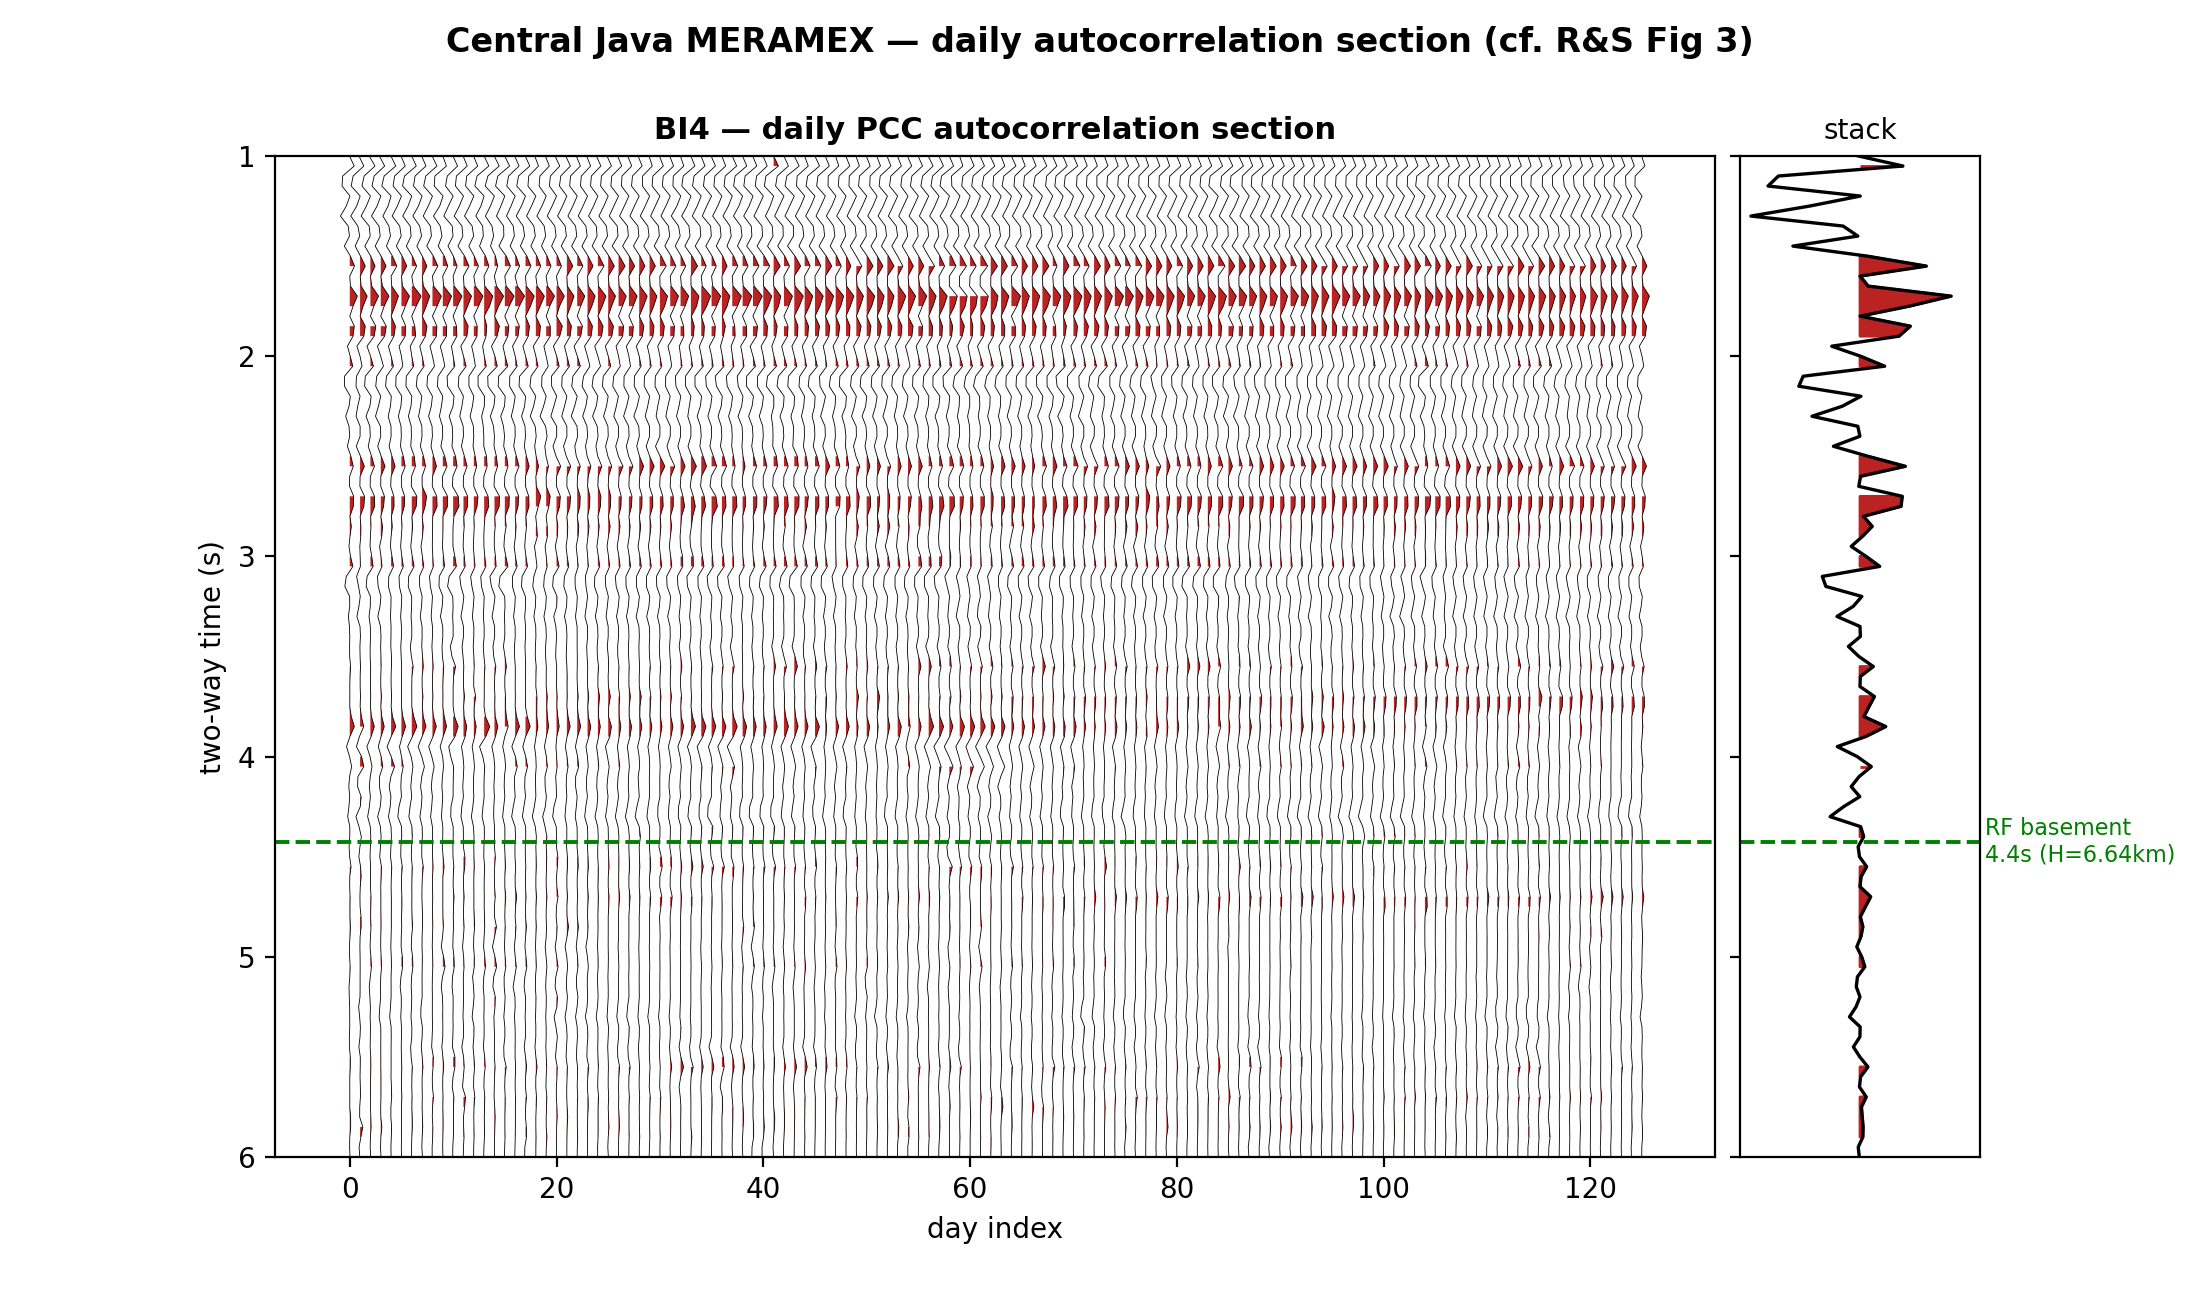
\includegraphics[width=0.95\textwidth]{rs_fig3_section.png}
\caption{Daily ambient-noise autocorrelation section at a representative station
(phase cross-correlation + phase-weighted stack), displayed from 1~s two-way time
upward after \citet{Romero2018}. The basement P reflection appears as a
day-stable, band-stable arrival; the multi-band test rejects the common zero-lag
side lobe.}
\label{fig:acsection}
\end{figure}

\begin{figure}[p]\centering
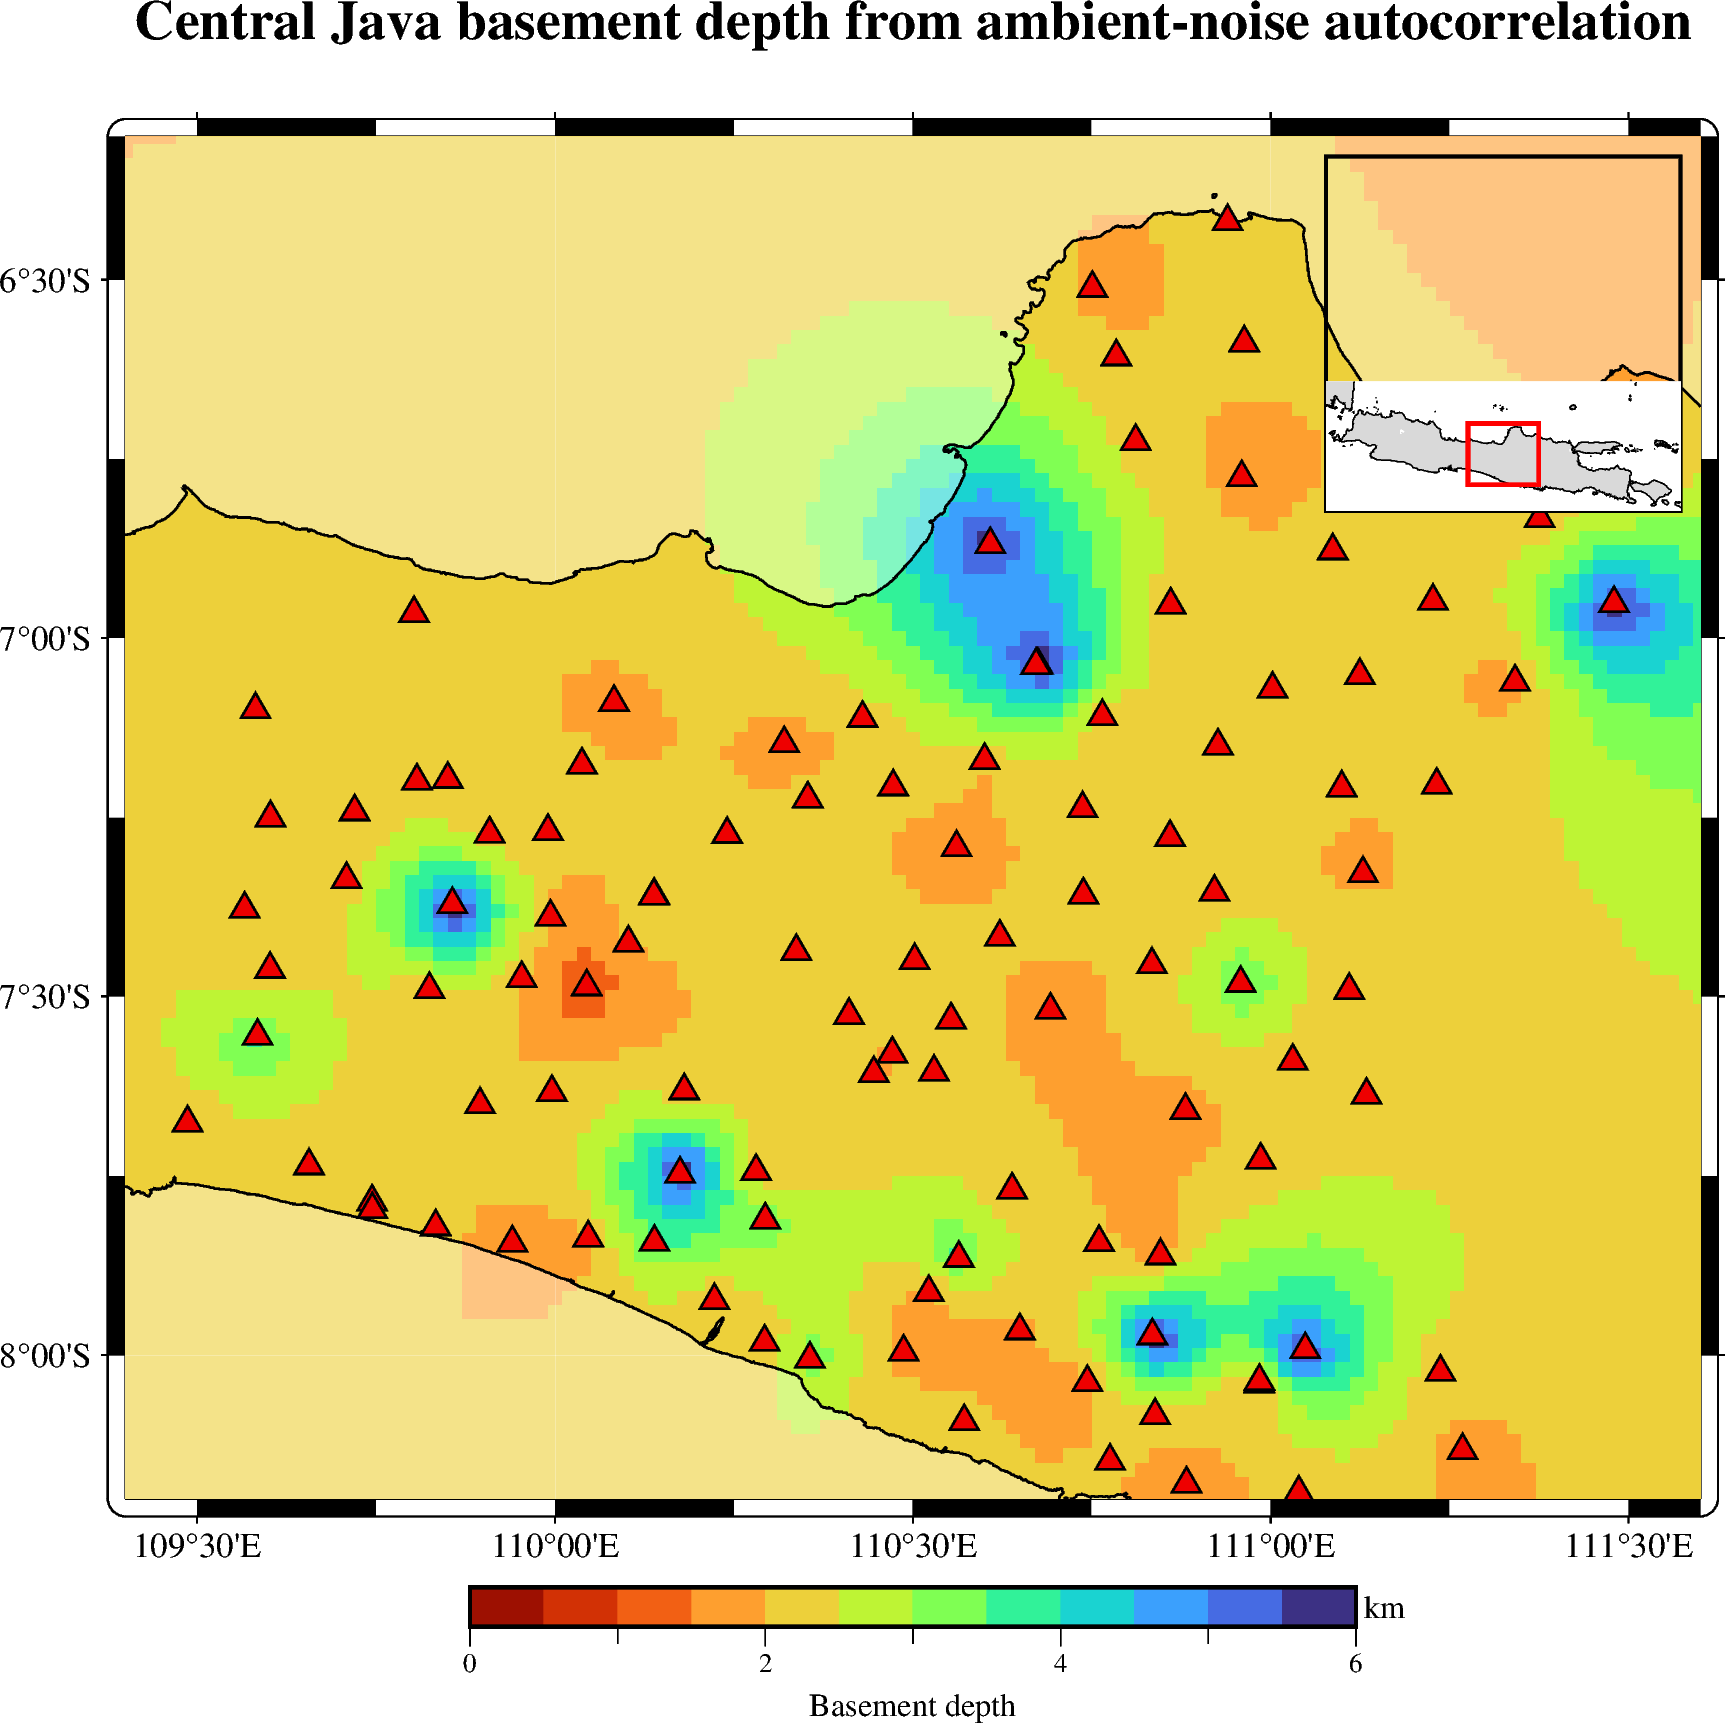
\includegraphics[width=\textwidth]{basement_map_an.png}
\caption{Receiver-function-\emph{independent} basement-depth map from ambient-noise
autocorrelation (111 stations, median $2.1$~km, range $0.9$--$8.8$~km), drawn in
the \citet{Romero2018} style. It reproduces the deep axis of the RF and
anchored-gravity models using no receiver-function information.}
\label{fig:anmap}
\end{figure}

\begin{figure}[p]\centering
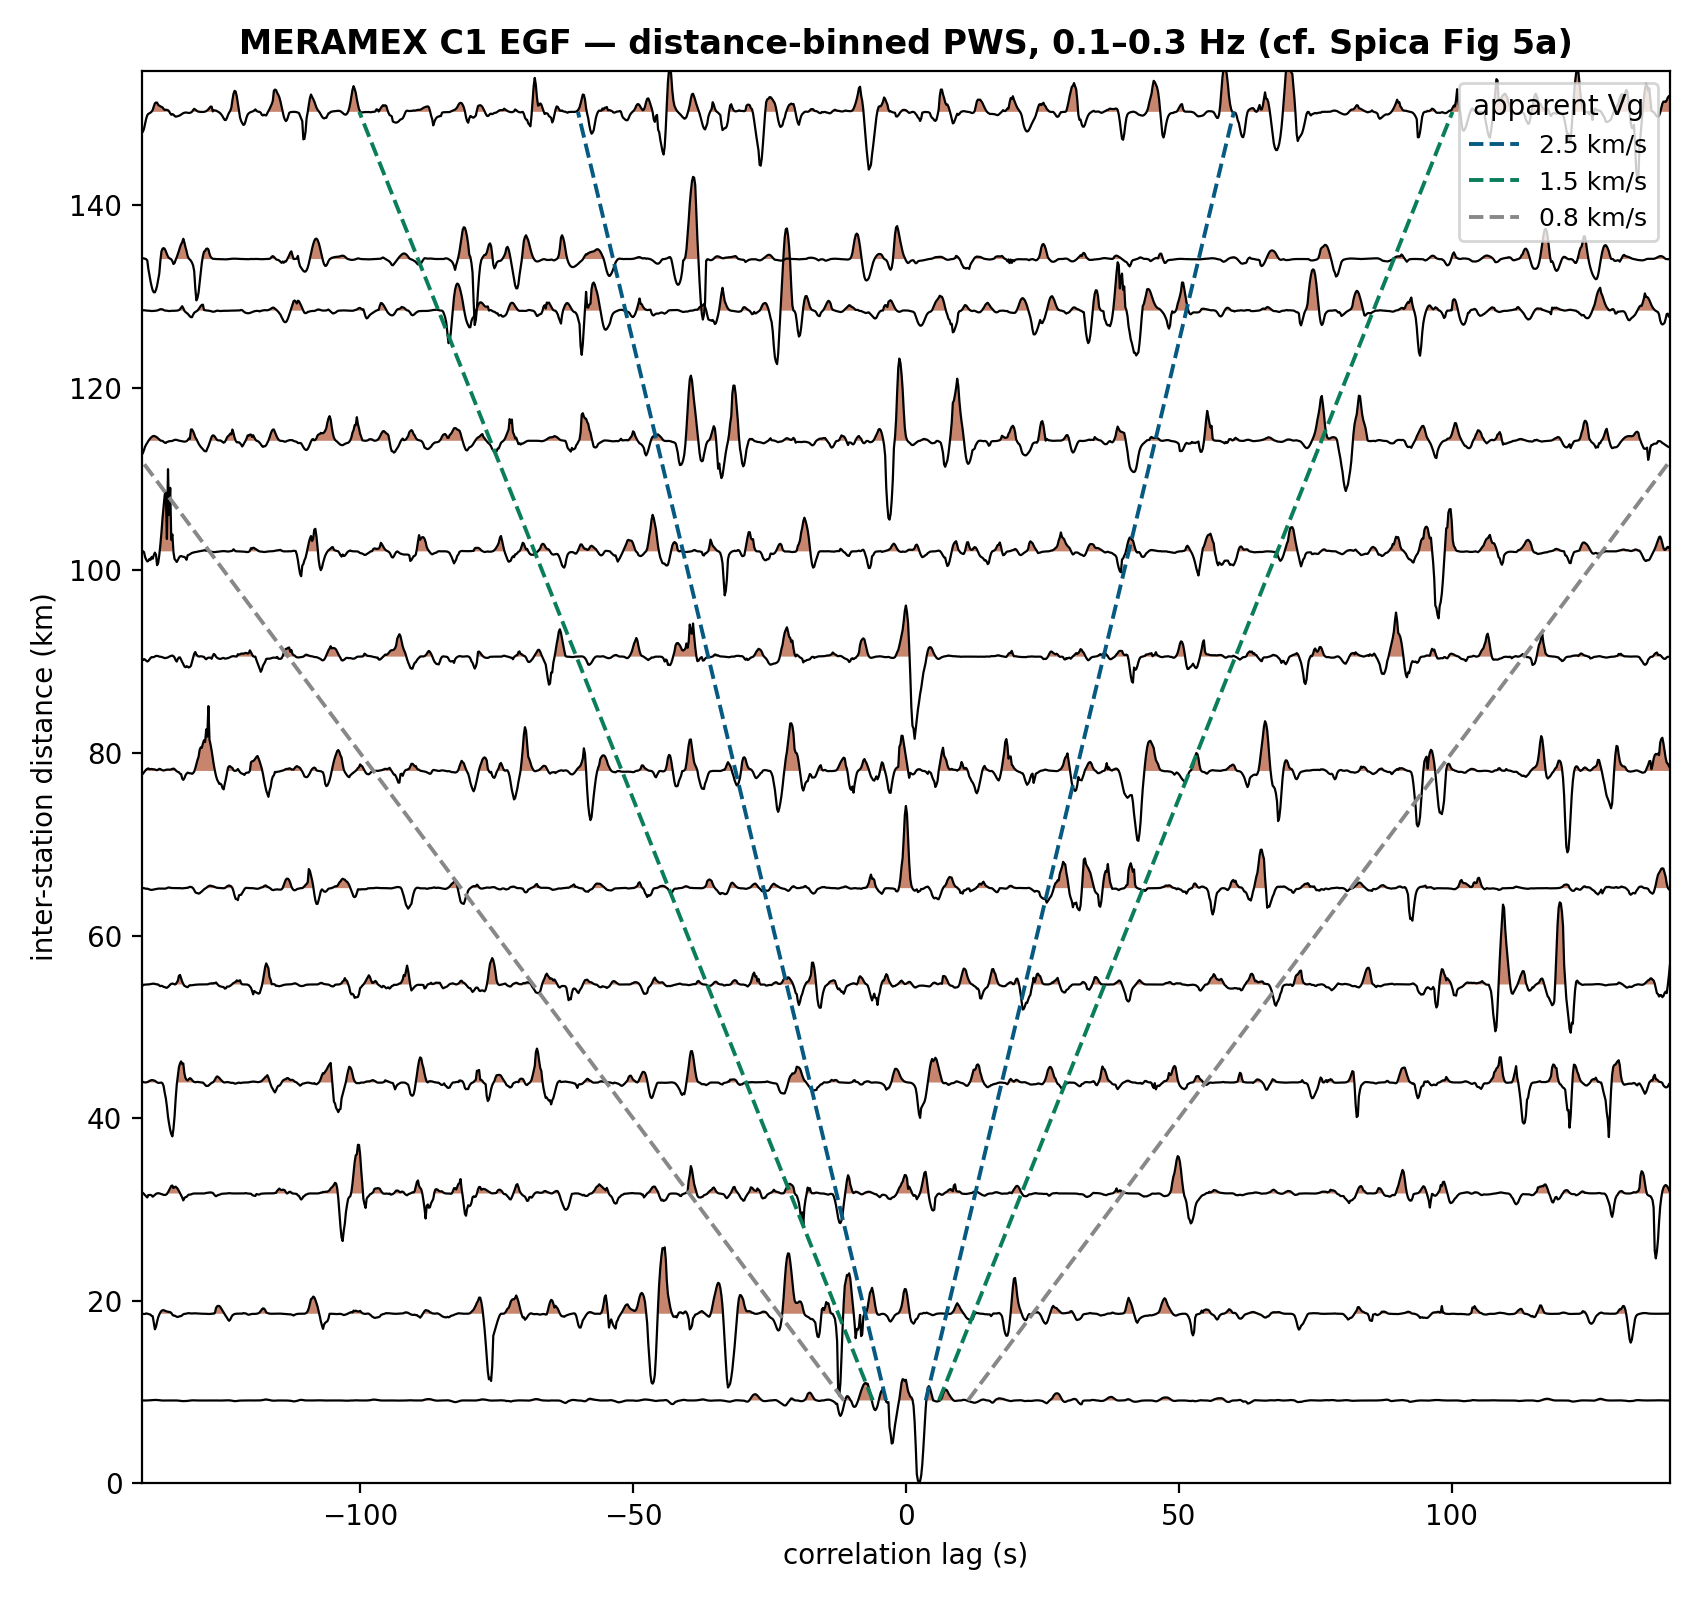
\includegraphics[width=0.49\textwidth]{spica_record_section.png}\hfill
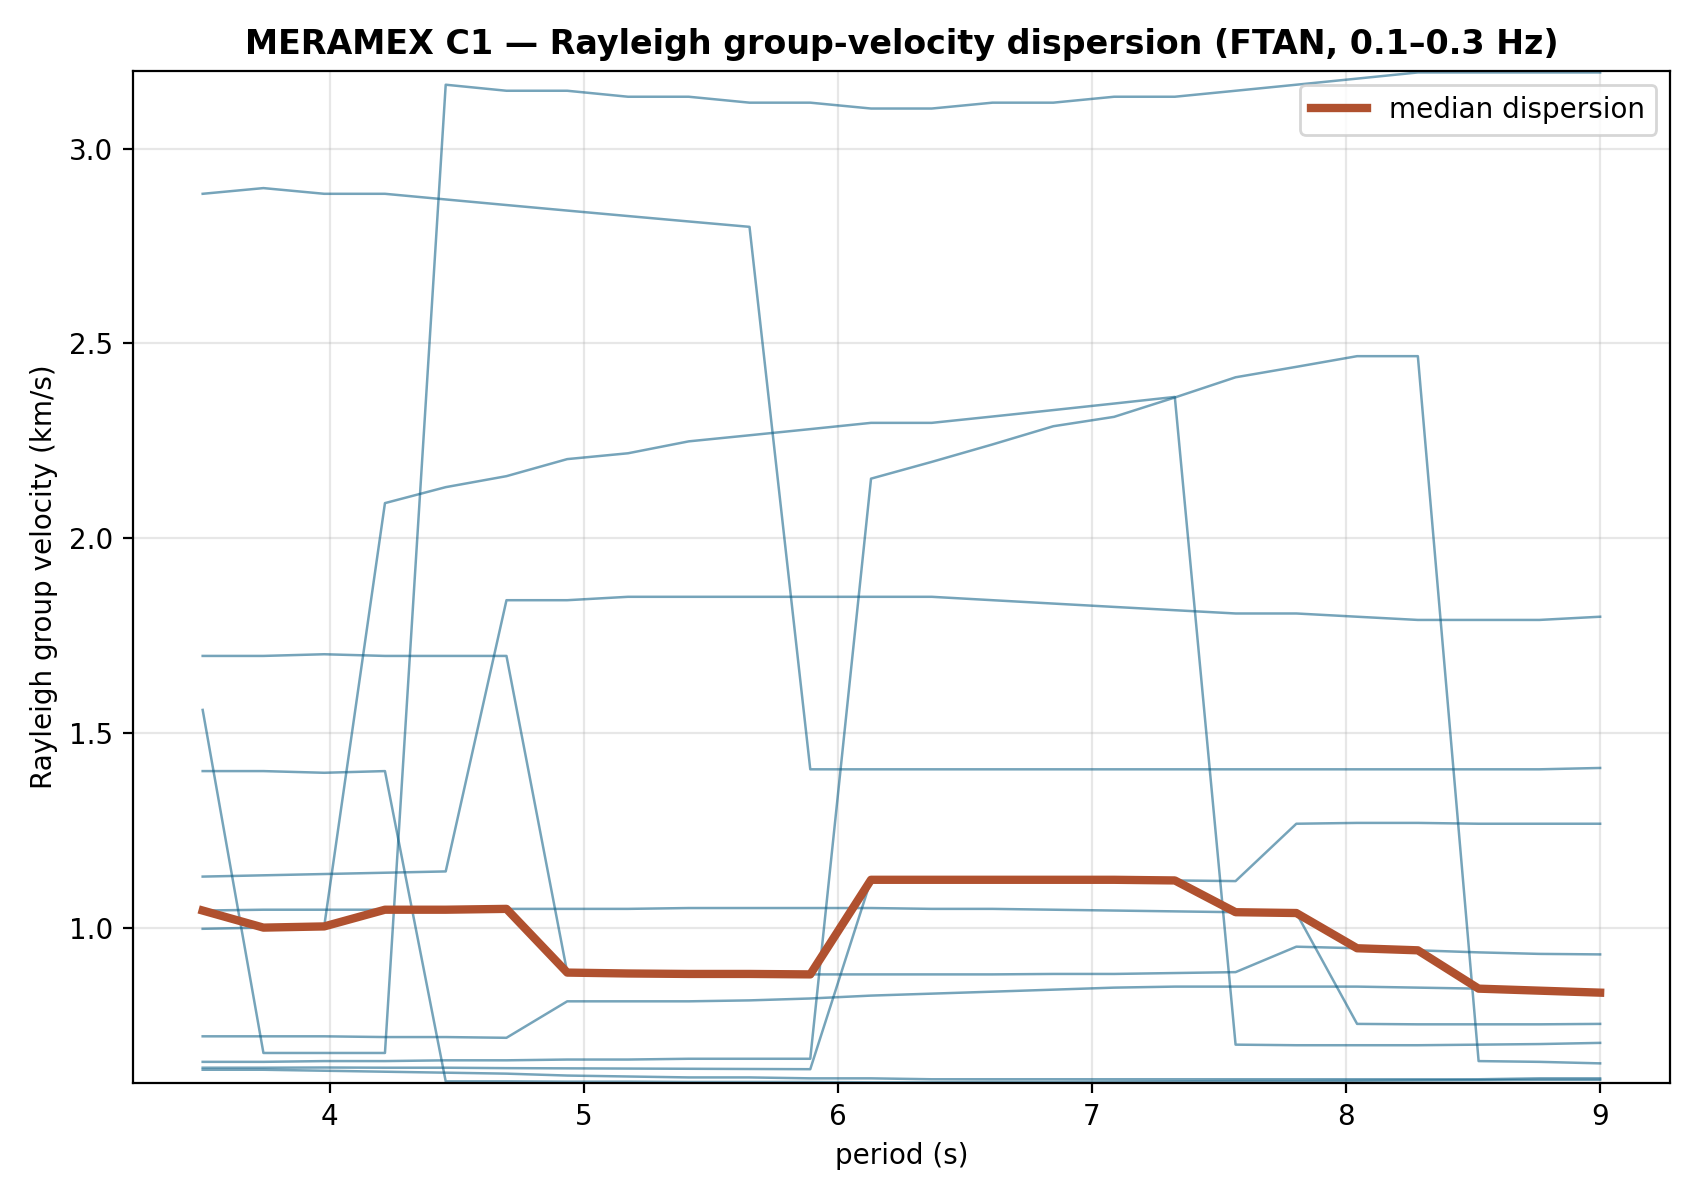
\includegraphics[width=0.49\textwidth]{spica_dispersion.png}
\caption{Ambient-noise cross-correlation (C1), all days, microseism band
($0.1$--$0.3$~\si{\hertz}), phase-weighted stack. (a) Distance-binned EGF record
section with Rayleigh move-out; (b) FTAN group-velocity dispersion, clustering
near $\sim$1~\si{\km\per\s} (soft fill) but resolution-limited by the short-period
array.}
\label{fig:spica}
\end{figure}

\begin{figure}[p]\centering
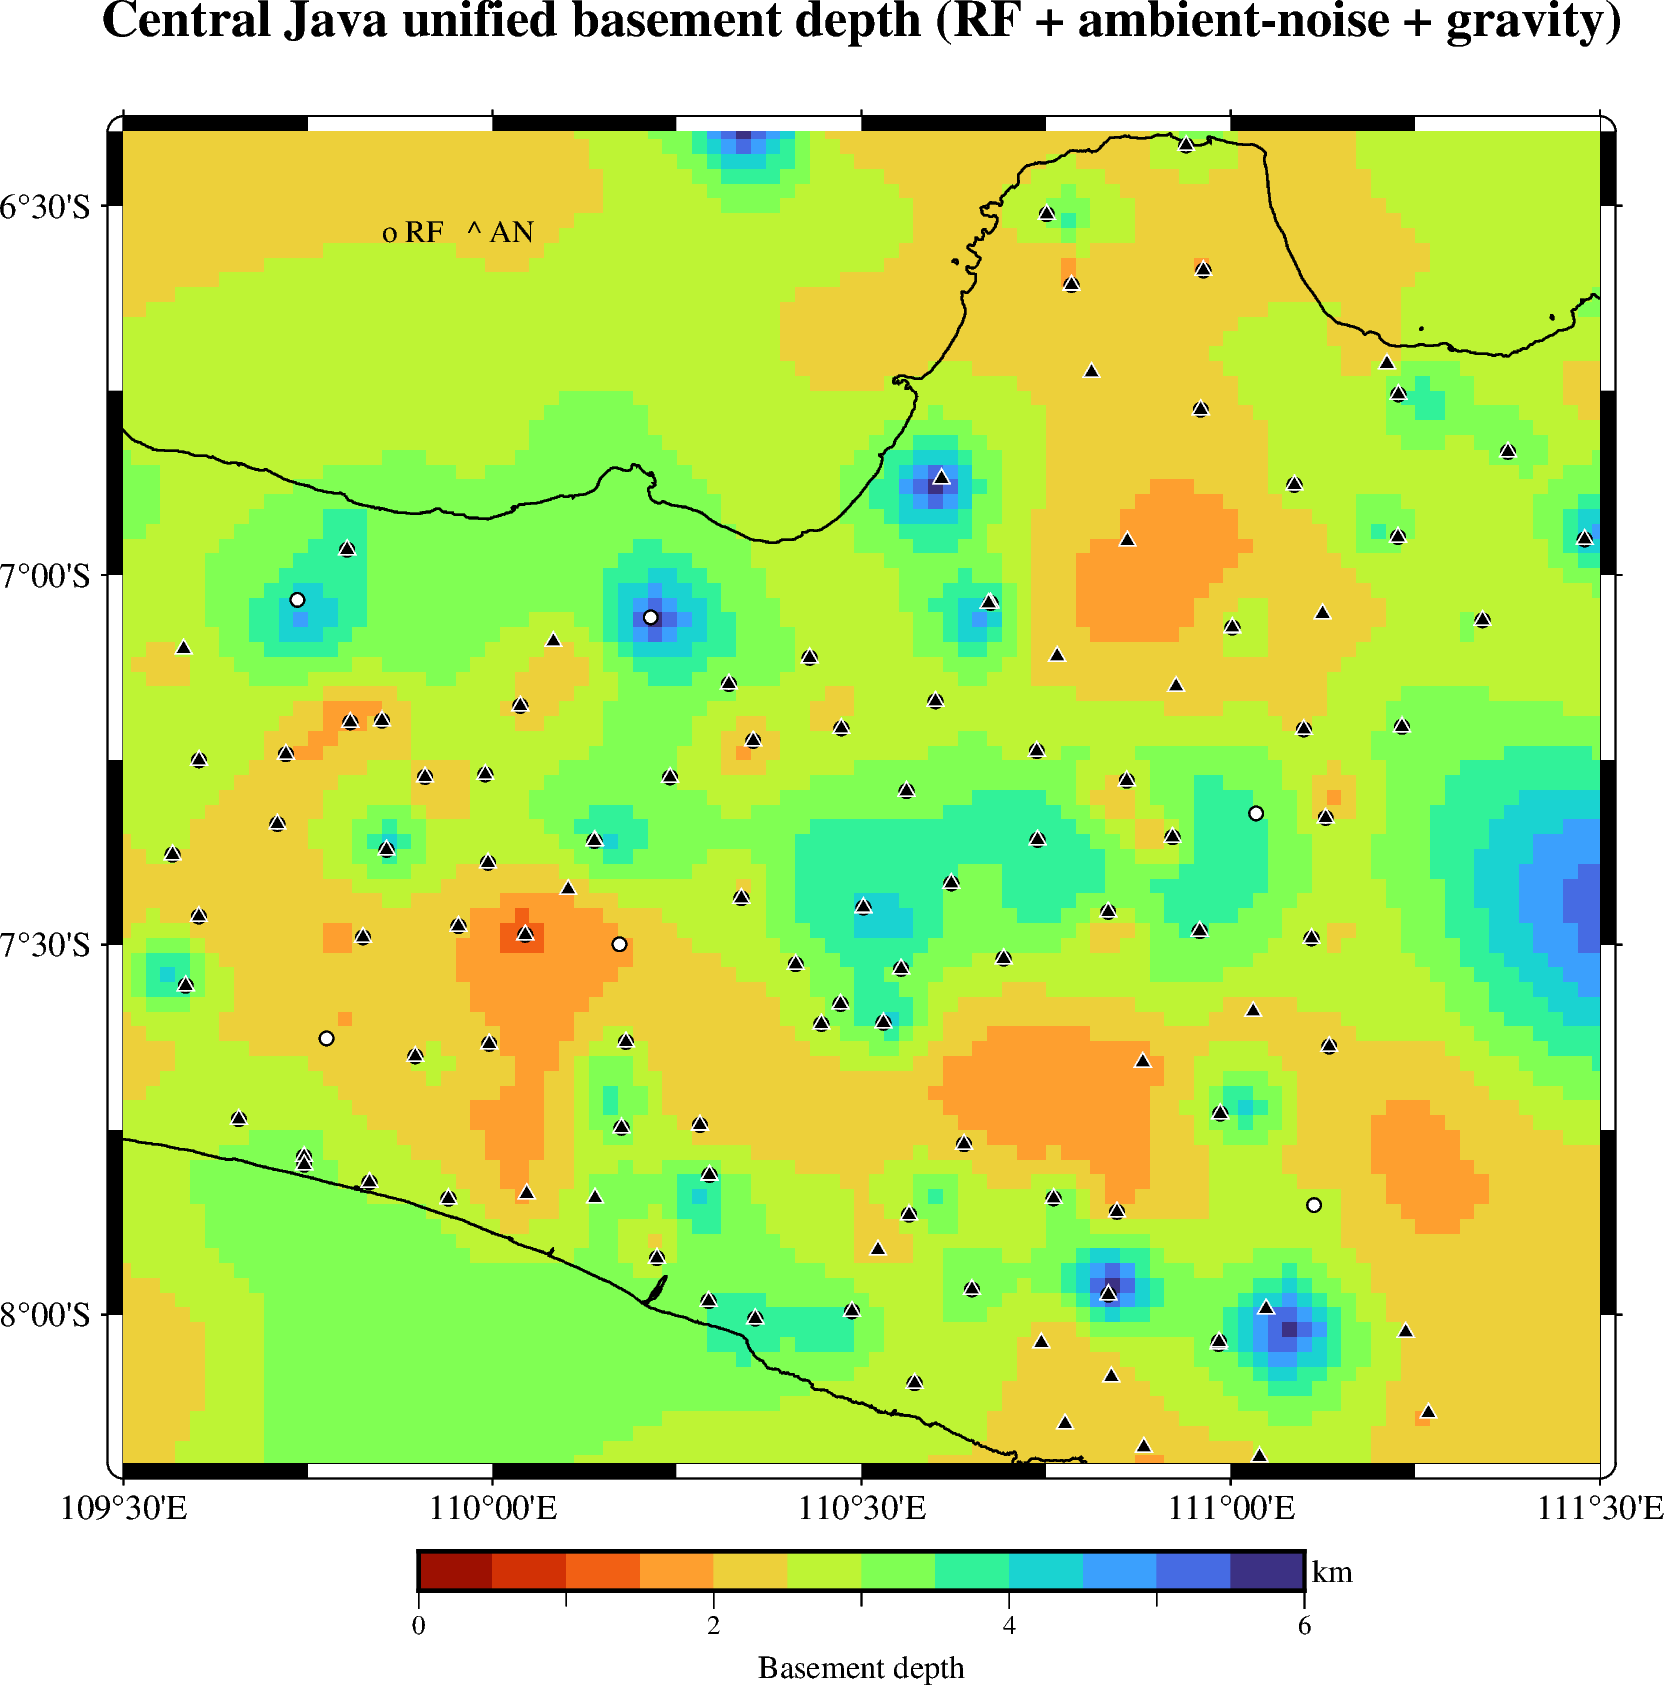
\includegraphics[width=\textwidth]{joint_basement_map.png}
\caption{Joint RF\,+\,autocorrelation\,+\,gravity basement model
(Eq.~\ref{eq:joint}): a single grid (median $2.7$~km, range $1.2$--$5.4$~km)
consistent with both seismic estimates and interpolated by the gravity field.}
\label{fig:jointmap}
\end{figure}

\begin{figure}[p]\centering
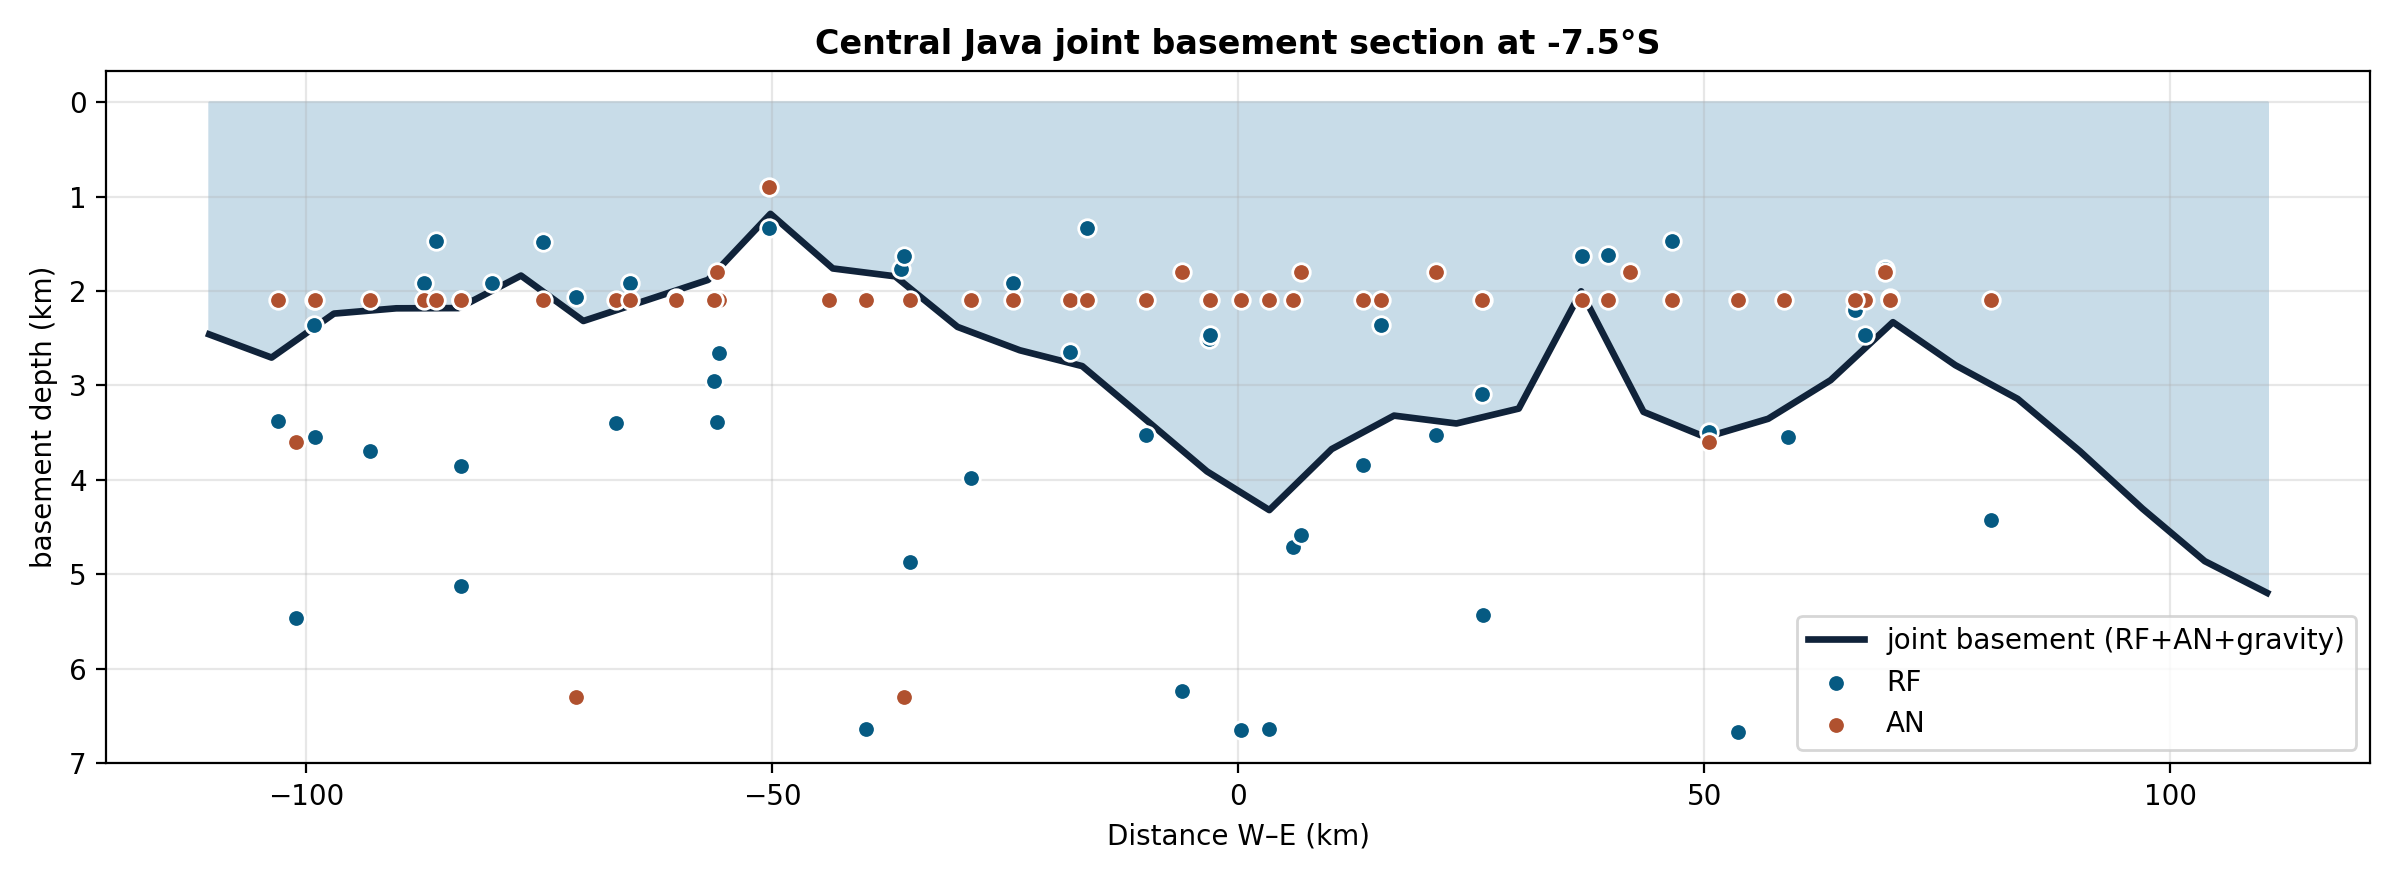
\includegraphics[width=\textwidth]{joint_section.png}
\caption{Cross-section through the joint basement model, showing the depocentre
geometry reconciled from reflection depths and gravity.}
\label{fig:jointsection}
\end{figure}

\begin{figure}[p]\centering
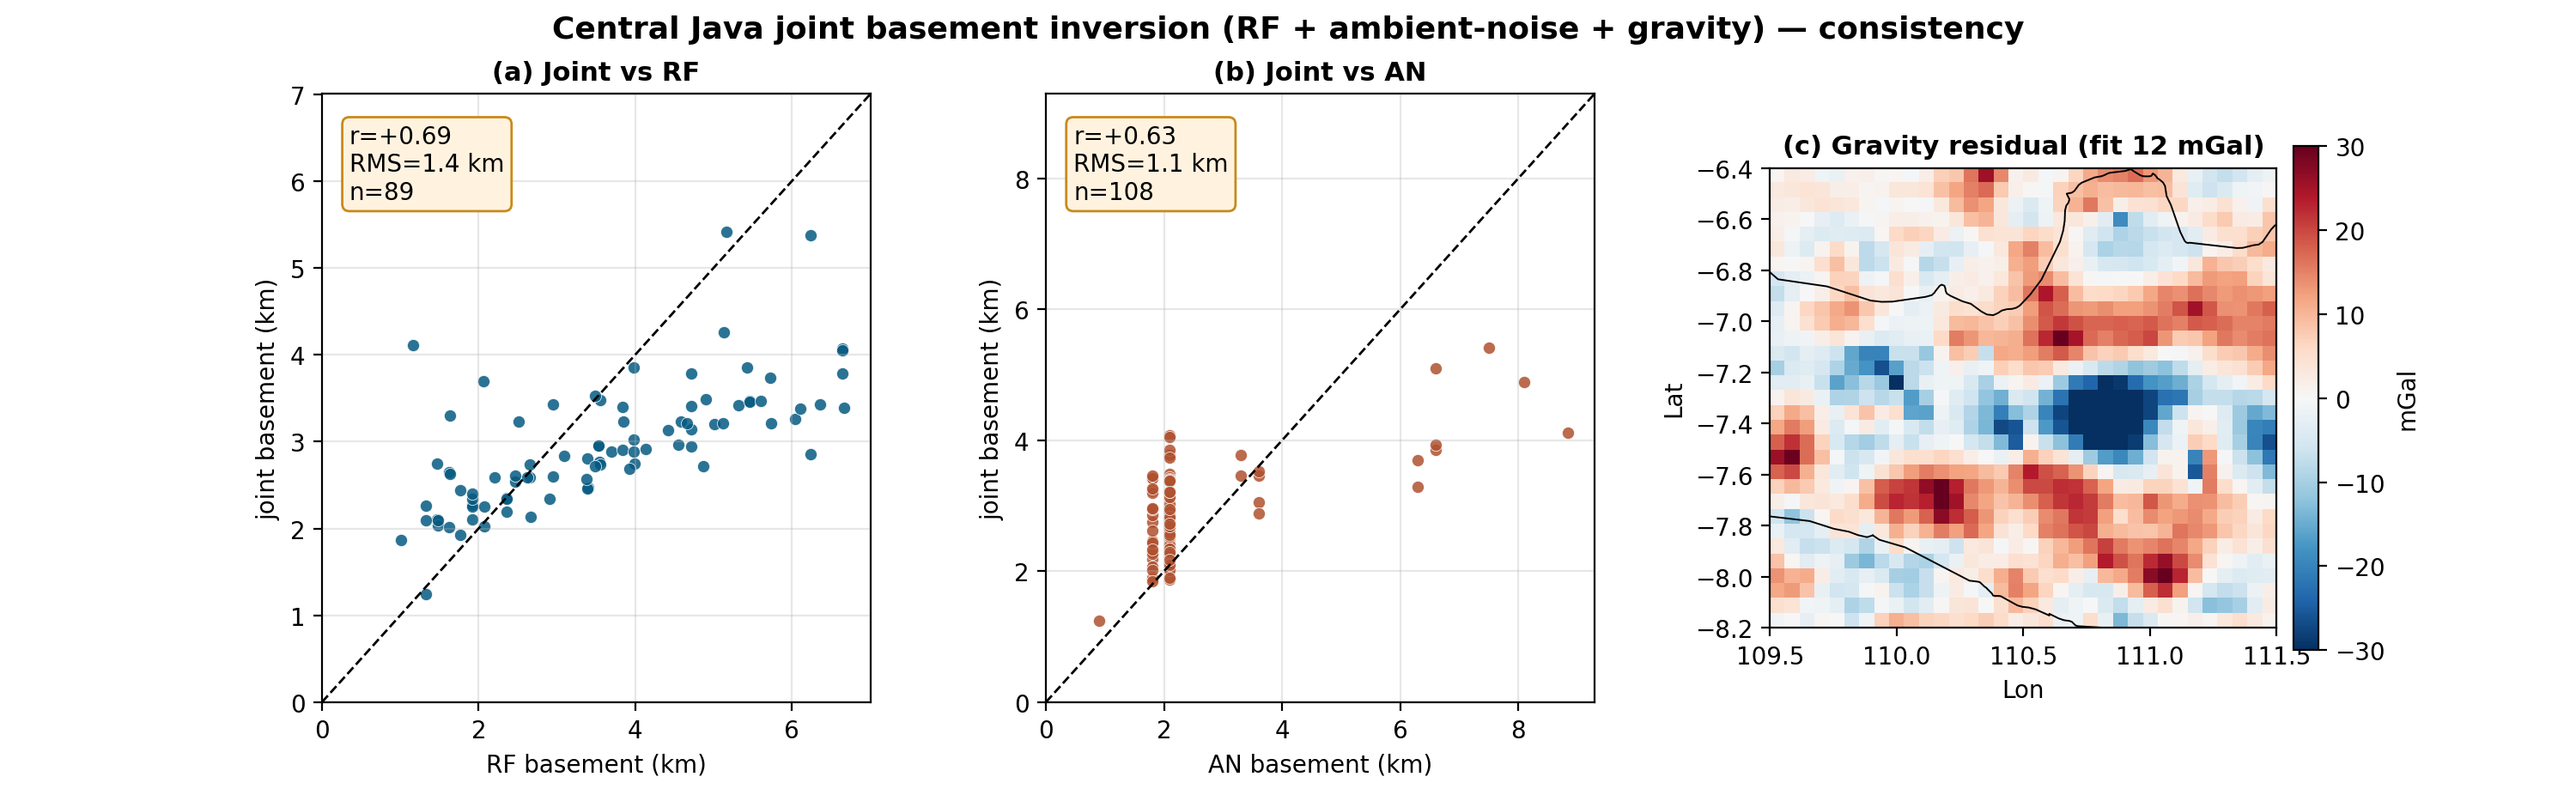
\includegraphics[width=0.8\textwidth]{joint_scatter.png}
\caption{Consistency of the joint model with its seismic inputs: joint basement
depth versus receiver-function depth ($r=0.69$) and versus autocorrelation depth
($r=0.63$).}
\label{fig:jointscatter}
\end{figure}

\begin{figure}[p]\centering
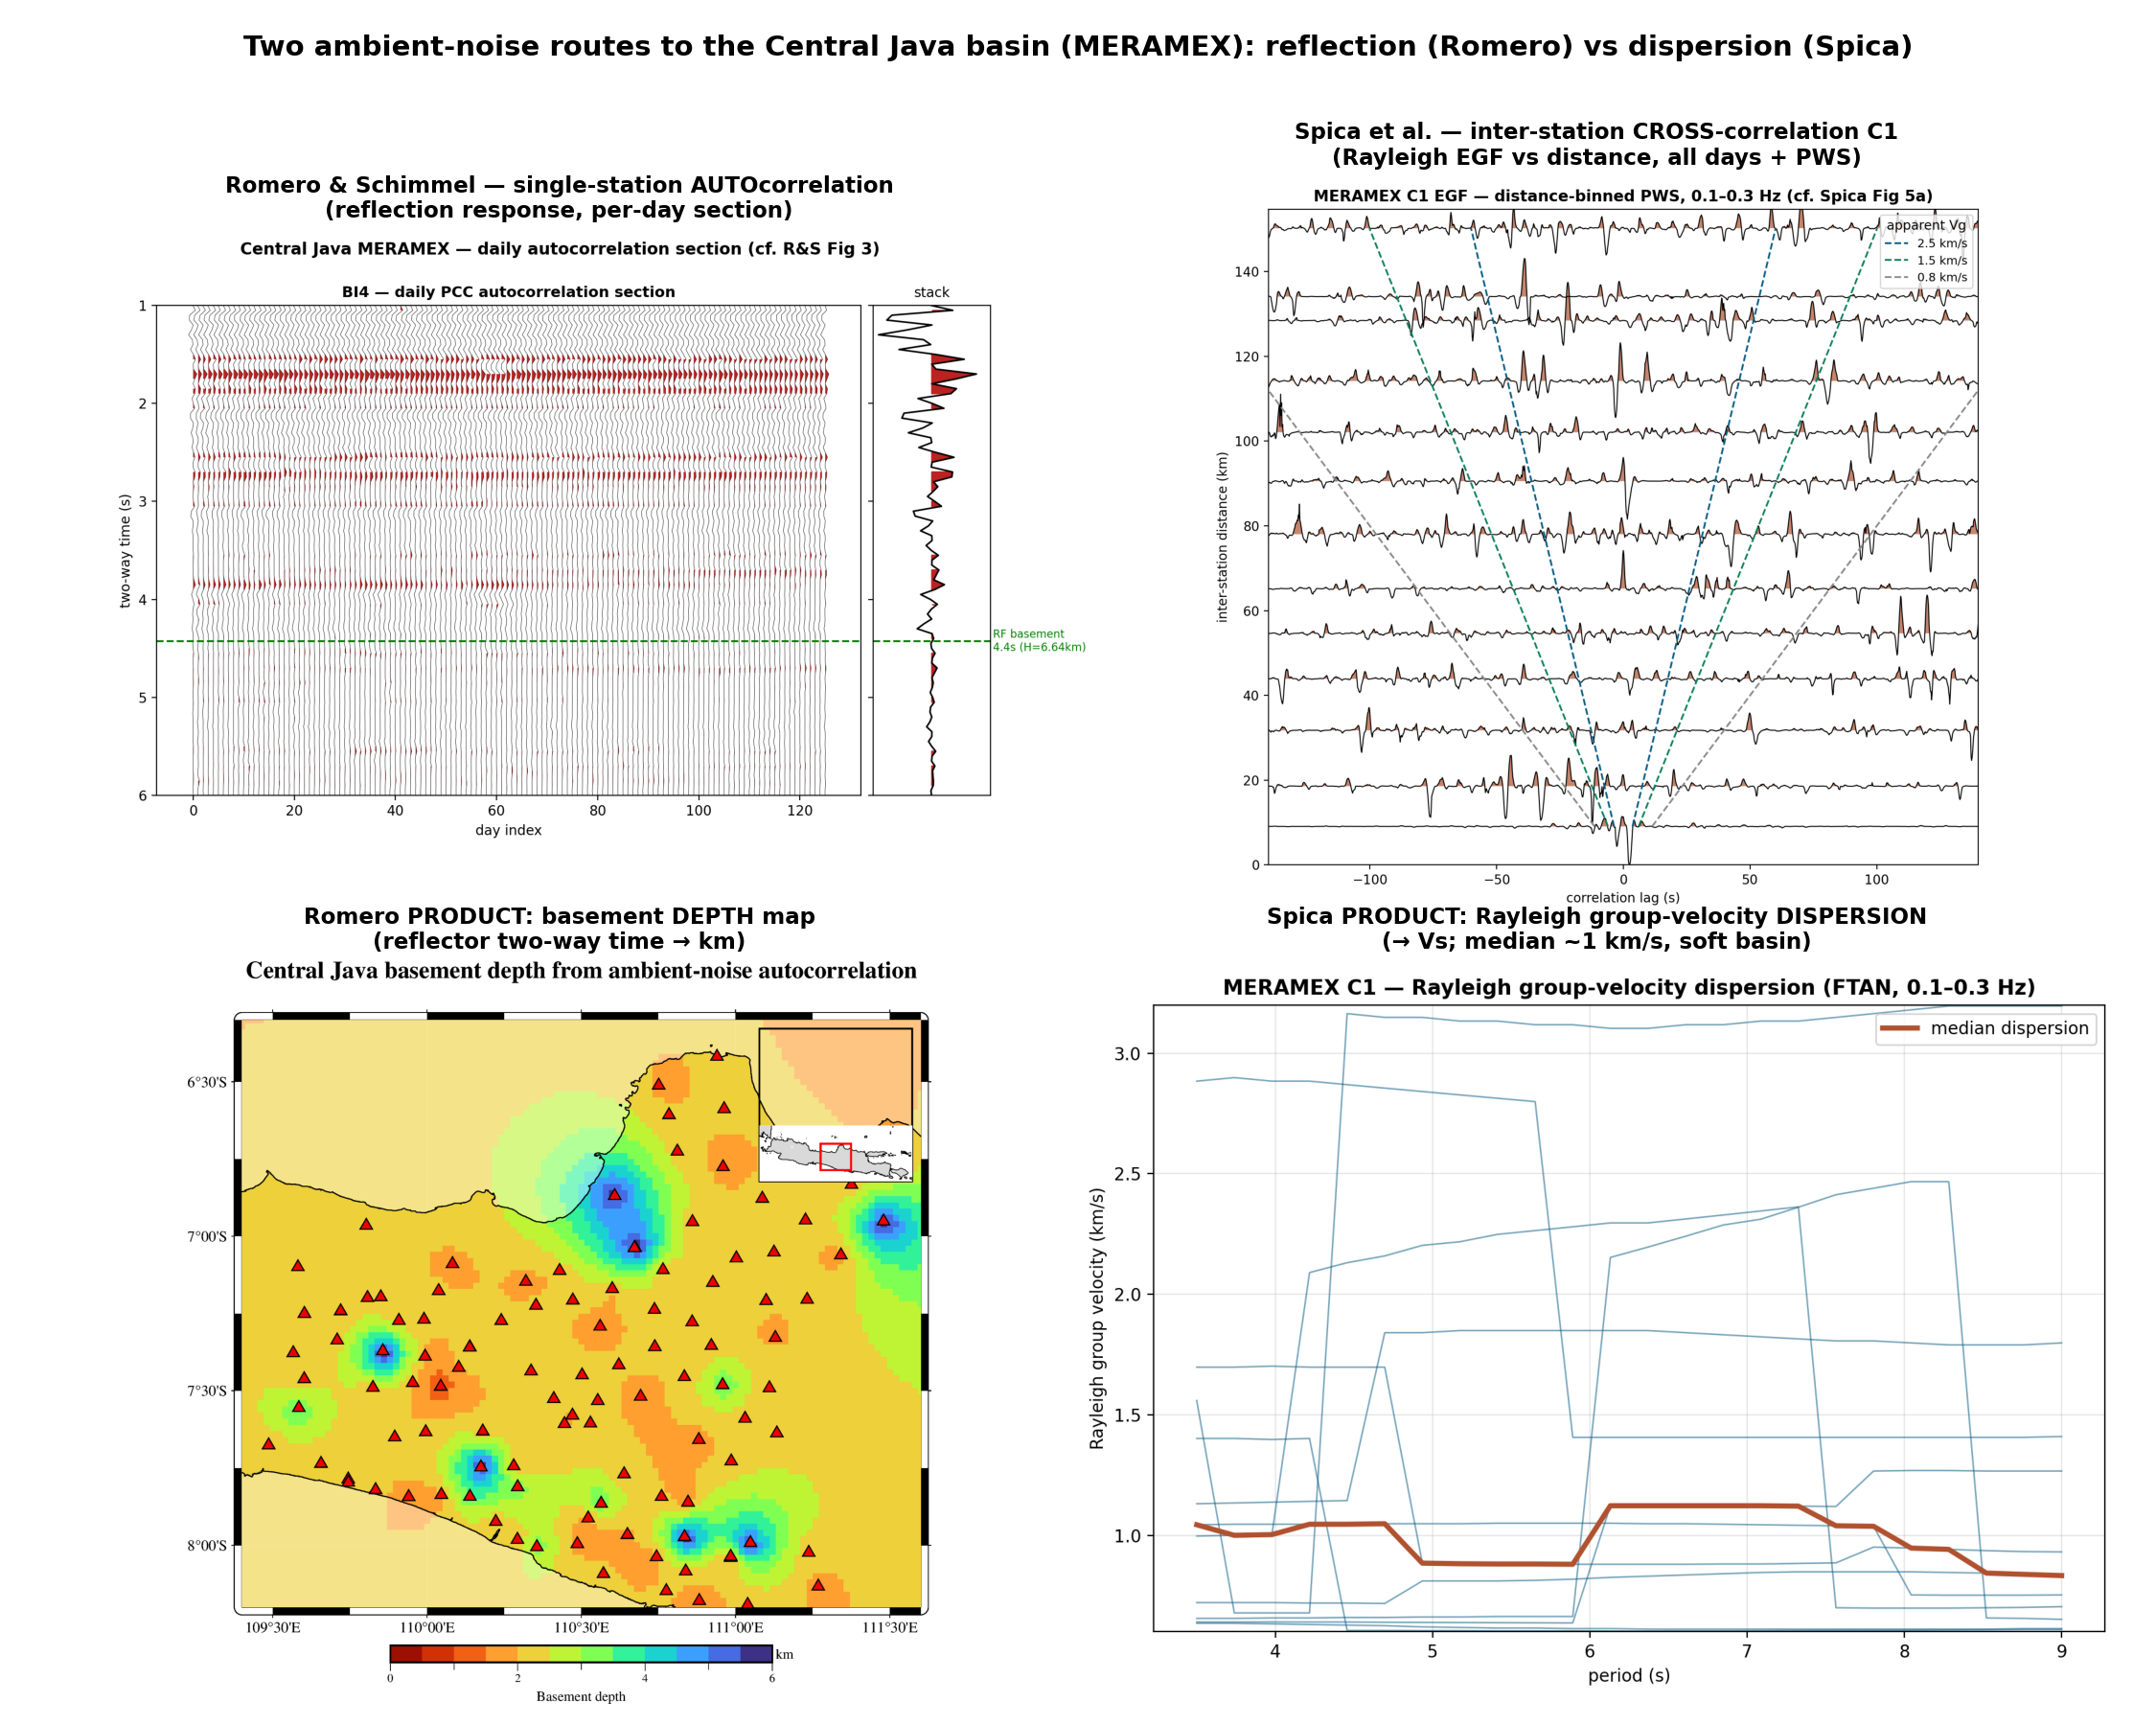
\includegraphics[width=\textwidth]{compare_romero_spica.png}
\caption{The two ambient-noise routes side by side: autocorrelation
\citep{Romero2018} delivers absolute reflector depth, cross-correlation
\citep{Spica2016} delivers shallow velocity --- complementary constraints on the
same basin.}
\label{fig:compare}
\end{figure}

\end{document}
